\chapter{Results} \label{cap:result}

In this chapter, we present the results of the various machine learning
approaches used to train the models discussed in Chapter
\ref{cap:contrib}. These results are presented using tables and visualizations
to facilitate understanding the benefits and limitations of each decision. The
tables and visualizations, provide a concise and comparative summary of the
performance metrics, such as accuracy, AUC and recall. \\

Additionally, we showcase the outcomes of the CAD infrastructure constructed
around this thesis.


\section{Metrics}

After training each model and inferring the predictions, we saved the metrics
of interest for each dataset (train, validate, test). The training information
of each training approach is given in Table
\ref{table:trained-models-information}. On the other hand, Table
\ref{table:resume-metrics} provides a summary of the metrics acquired for each
model in the different datasets. \\

The accuracy metric in Table \ref{table:resume-metrics} represents the
overall performance of the model in the multi-class classification problem with
8 different labels. However, as unbalanced multi-class problem, accuracy may not
be the most suitable metric to assess the model's performance in this
situation. Instead, metrics like AUC (Area Under the Curve) and recall should
be considered, as they specifically indicate how well the model is performing
in classifying melanoma from the other classes. \\

The metrics with a gray background in Table \ref{table:resume-metrics}
are from models that incorporated additional regularization techniques, such as
dropout or data augmentation. These models were trained for 40 epochs since
regularization tends to slow down the minimization of the objective function
compared to the other models that were trained for only 20 epochs. \\

To facilitate a better comparison between the two approaches, we computed the
mean and standard deviation for each training approach.

\newpage

It is important to mention that the metrics obtained for all models, both on
the validation and test sets, were generated using the Test-Time Augmentation
technique. As explained in previous chapters, this technique functions as an
ensemble, contributing to improved performance during inference. \\

Models that used a scheduler during the training stage are denoted with a
symbol next to their names. For reference, the mapping between the scheduler
used and the corresponding symbol is provided in Table
\ref{table:scheduler-mapping}.

\begin{table}[H]
  \centering
  \begin{tabular}{cc}
    \toprule
    \multicolumn{2}{c}{\textbf{Scheduler Mapping}} \\
    \midrule
    $\star$     & Step Learning Rate \\
    $\ast$      & Cosine Annealing Learning Rate \\
    $\bullet$   & Cosine Annealing Warm Restarts \\
    \bottomrule
  \end{tabular}
  \caption[Scheduler Mapping]
  {\textit{Scheduler Mapping.}}
  \label{table:scheduler-mapping}
\end{table}

\newpage

\begin{landscape}

  \begin{table}
    \centering
    \begin{tabular}{lccccccccc}
      \toprule
      & \textbf{Train AUC} & \textbf{Val AUC} & \textbf{Test AUC} & \textbf{Train Recall} & \textbf{Val Recall} & \textbf{Test Recall} & \textbf{Train Acc} & \textbf{Val Acc} & \textbf{Test Acc} \\
      \midrule
      M0 & 0.952 & 0.903 & 0.892 & 0.756 & 0.676 & 0.652 & 0.835 & 0.778 & 0.772 \\
      M1 $\star$ & 0.947 & 0.900 & 0.892 & 0.695 & 0.633 & 0.599 & 0.829 & 0.779 & 0.771 \\
      M2 $\ast$ & 0.933 & 0.895 & 0.885 & 0.658 & 0.609 & 0.582 & 0.808 & 0.765 & 0.762 \\
      M3 $\bullet$ & 0.935 & 0.896 & 0.886 & 0.663 & 0.605 & 0.589 & 0.811 & 0.767 & 0.764 \\
      \midrule
      \cellcolor{gray!50}M4 & \cellcolor{gray!50}0.886 & \cellcolor{gray!50}0.877 & \cellcolor{gray!50}0.858 & \cellcolor{gray!50}0.478 & \cellcolor{gray!50}0.475 & \cellcolor{gray!50}0.446 & \cellcolor{gray!50}0.757 & \cellcolor{gray!50}0.750 & \cellcolor{gray!50}0.741 \\
      \cellcolor{gray!50}M5 $\star$ & \cellcolor{gray!50}0.867 & \cellcolor{gray!50}0.861 & \cellcolor{gray!50}0.843 & \cellcolor{gray!50}0.423 & \cellcolor{gray!50}0.403 & \cellcolor{gray!50}0.395 & \cellcolor{gray!50}0.728 & \cellcolor{gray!50}0.717 &  \cellcolor{gray!50}0.715 \\
      \cellcolor{gray!50}M6 $\ast$ & \cellcolor{gray!50}0.874 & \cellcolor{gray!50}0.868 & \cellcolor{gray!50}0.848 & \cellcolor{gray!50}0.451 & \cellcolor{gray!50}0.440 & \cellcolor{gray!50}0.418 & \cellcolor{gray!50}0.738 & \cellcolor{gray!50}0.728 &  \cellcolor{gray!50}0.722 \\
      \cellcolor{gray!50}M7 $\bullet$ & \cellcolor{gray!50}0.877 & \cellcolor{gray!50}0.869 & \cellcolor{gray!50}0.849 & \cellcolor{gray!50}0.470 & \cellcolor{gray!50}0.458 & \cellcolor{gray!50}0.432 & \cellcolor{gray!50}0.742 & \cellcolor{gray!50}0.732 &  \cellcolor{gray!50}0.723 \\

      \midrule

      Mean &  94.175\% & 89.850\% & 88.875\%  & 69.300\% & 63.075\% & 60.550\% & 82.075\% & 77.225\% & 76.725\% \\
      SD   & 0.921\% & 0.370\% & 0.377\%  &  4.509\% & 3.260\% & 3.178\% & 1.327\% & 0.727\% & 0.499\% \\

      \midrule

      \cellcolor{gray!50}Mean & \cellcolor{gray!50}87.600\% & \cellcolor{gray!50}86.875\% & \cellcolor{gray!50}84.950\% & \cellcolor{gray!50}45.550\% & \cellcolor{gray!50}44.400\% & \cellcolor{gray!50}42.275\% & \cellcolor{gray!50}74.125\% & \cellcolor{gray!50}73.175\% & \cellcolor{gray!50}72.525\% \\
      \cellcolor{gray!50}SD & \cellcolor{gray!50}0.787\% & \cellcolor{gray!50}0.655\% & \cellcolor{gray!50}0.625\% & \cellcolor{gray!50}2.445\% & \cellcolor{gray!50}3.084\% & \cellcolor{gray!50}2.175\% & \cellcolor{gray!50}1.204\% & \cellcolor{gray!50}1.372\% &  \cellcolor{gray!50}1.108\% \\

      \bottomrule
    \end{tabular}
    \caption[Metrics in the Datasets]
    {\textit{Metrics in the Datasets. }}
    {\label{table:resume-metrics}}
  \end{table}

\end{landscape}


\section{Training}

In this section, we analyze the performance of the models throughout the
training process. Most of the graphics seen in this section were generated
using W\&B (Weight \& Biasses).\\


Every pair of models in the set \(S\), \(S=\{\{M0, M4\}, \{M2, M5\}, \{M3,
M6\}, \{M4, M8\}\}\), shares the same scheduler if they were used in the
training phase. However, each pair differs in batch size, the number of epochs,
and regularization techniques. \\

We are providing this comparison to demonstrate the impact of regularization on
the training process. It is evident that models trained for 20 epochs
experience overfitting due to the absence of regularization techniques. On the
other hand, models trained for 40 epochs do not suffer from overfitting, but
their performance is still inferior to models without additional
regularization. However, this issue probably can be resolved by increasing the
number of training epochs.

\subsection{M0 against M4}

\begin{figure}[H]
  \centering
  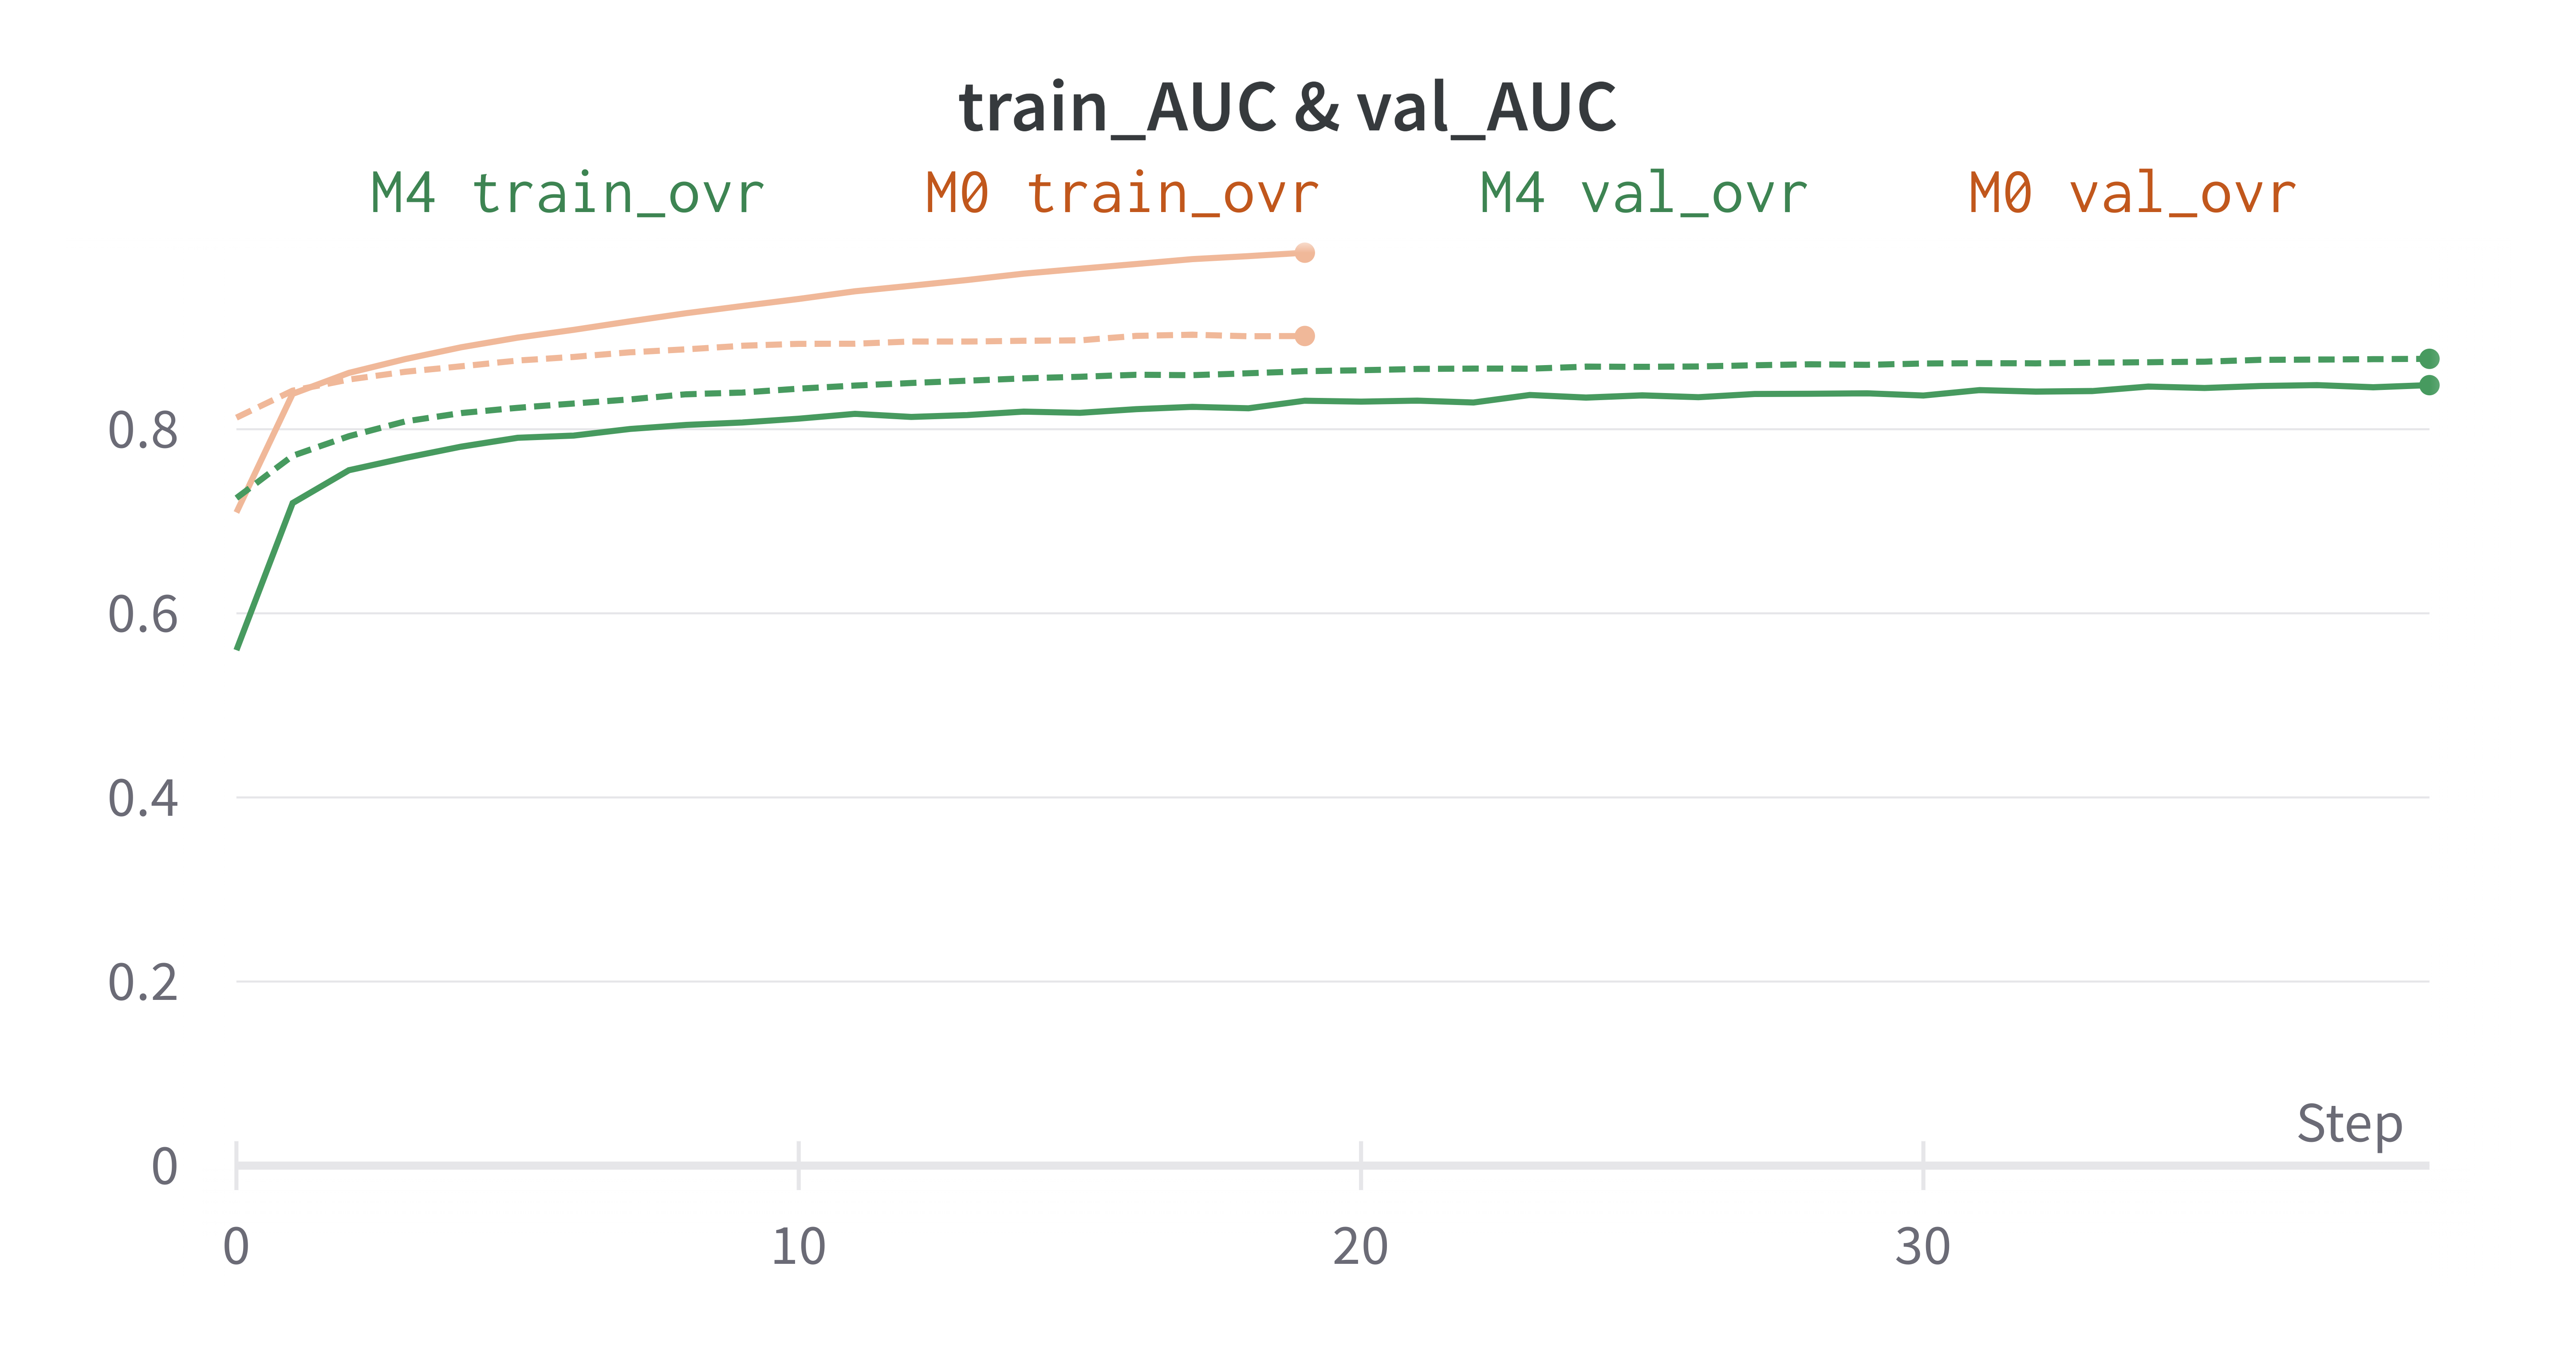
\includegraphics[width=\textwidth]{imatges/results/AUCM0M4.png}
  \caption[M0 vs. M4, AUC Train and Validation Curves]{\textit{M0 vs. M4, AUC Train and Validation Curves. }}
\end{figure}

\newpage

\begin{figure}[H]
  \centering
  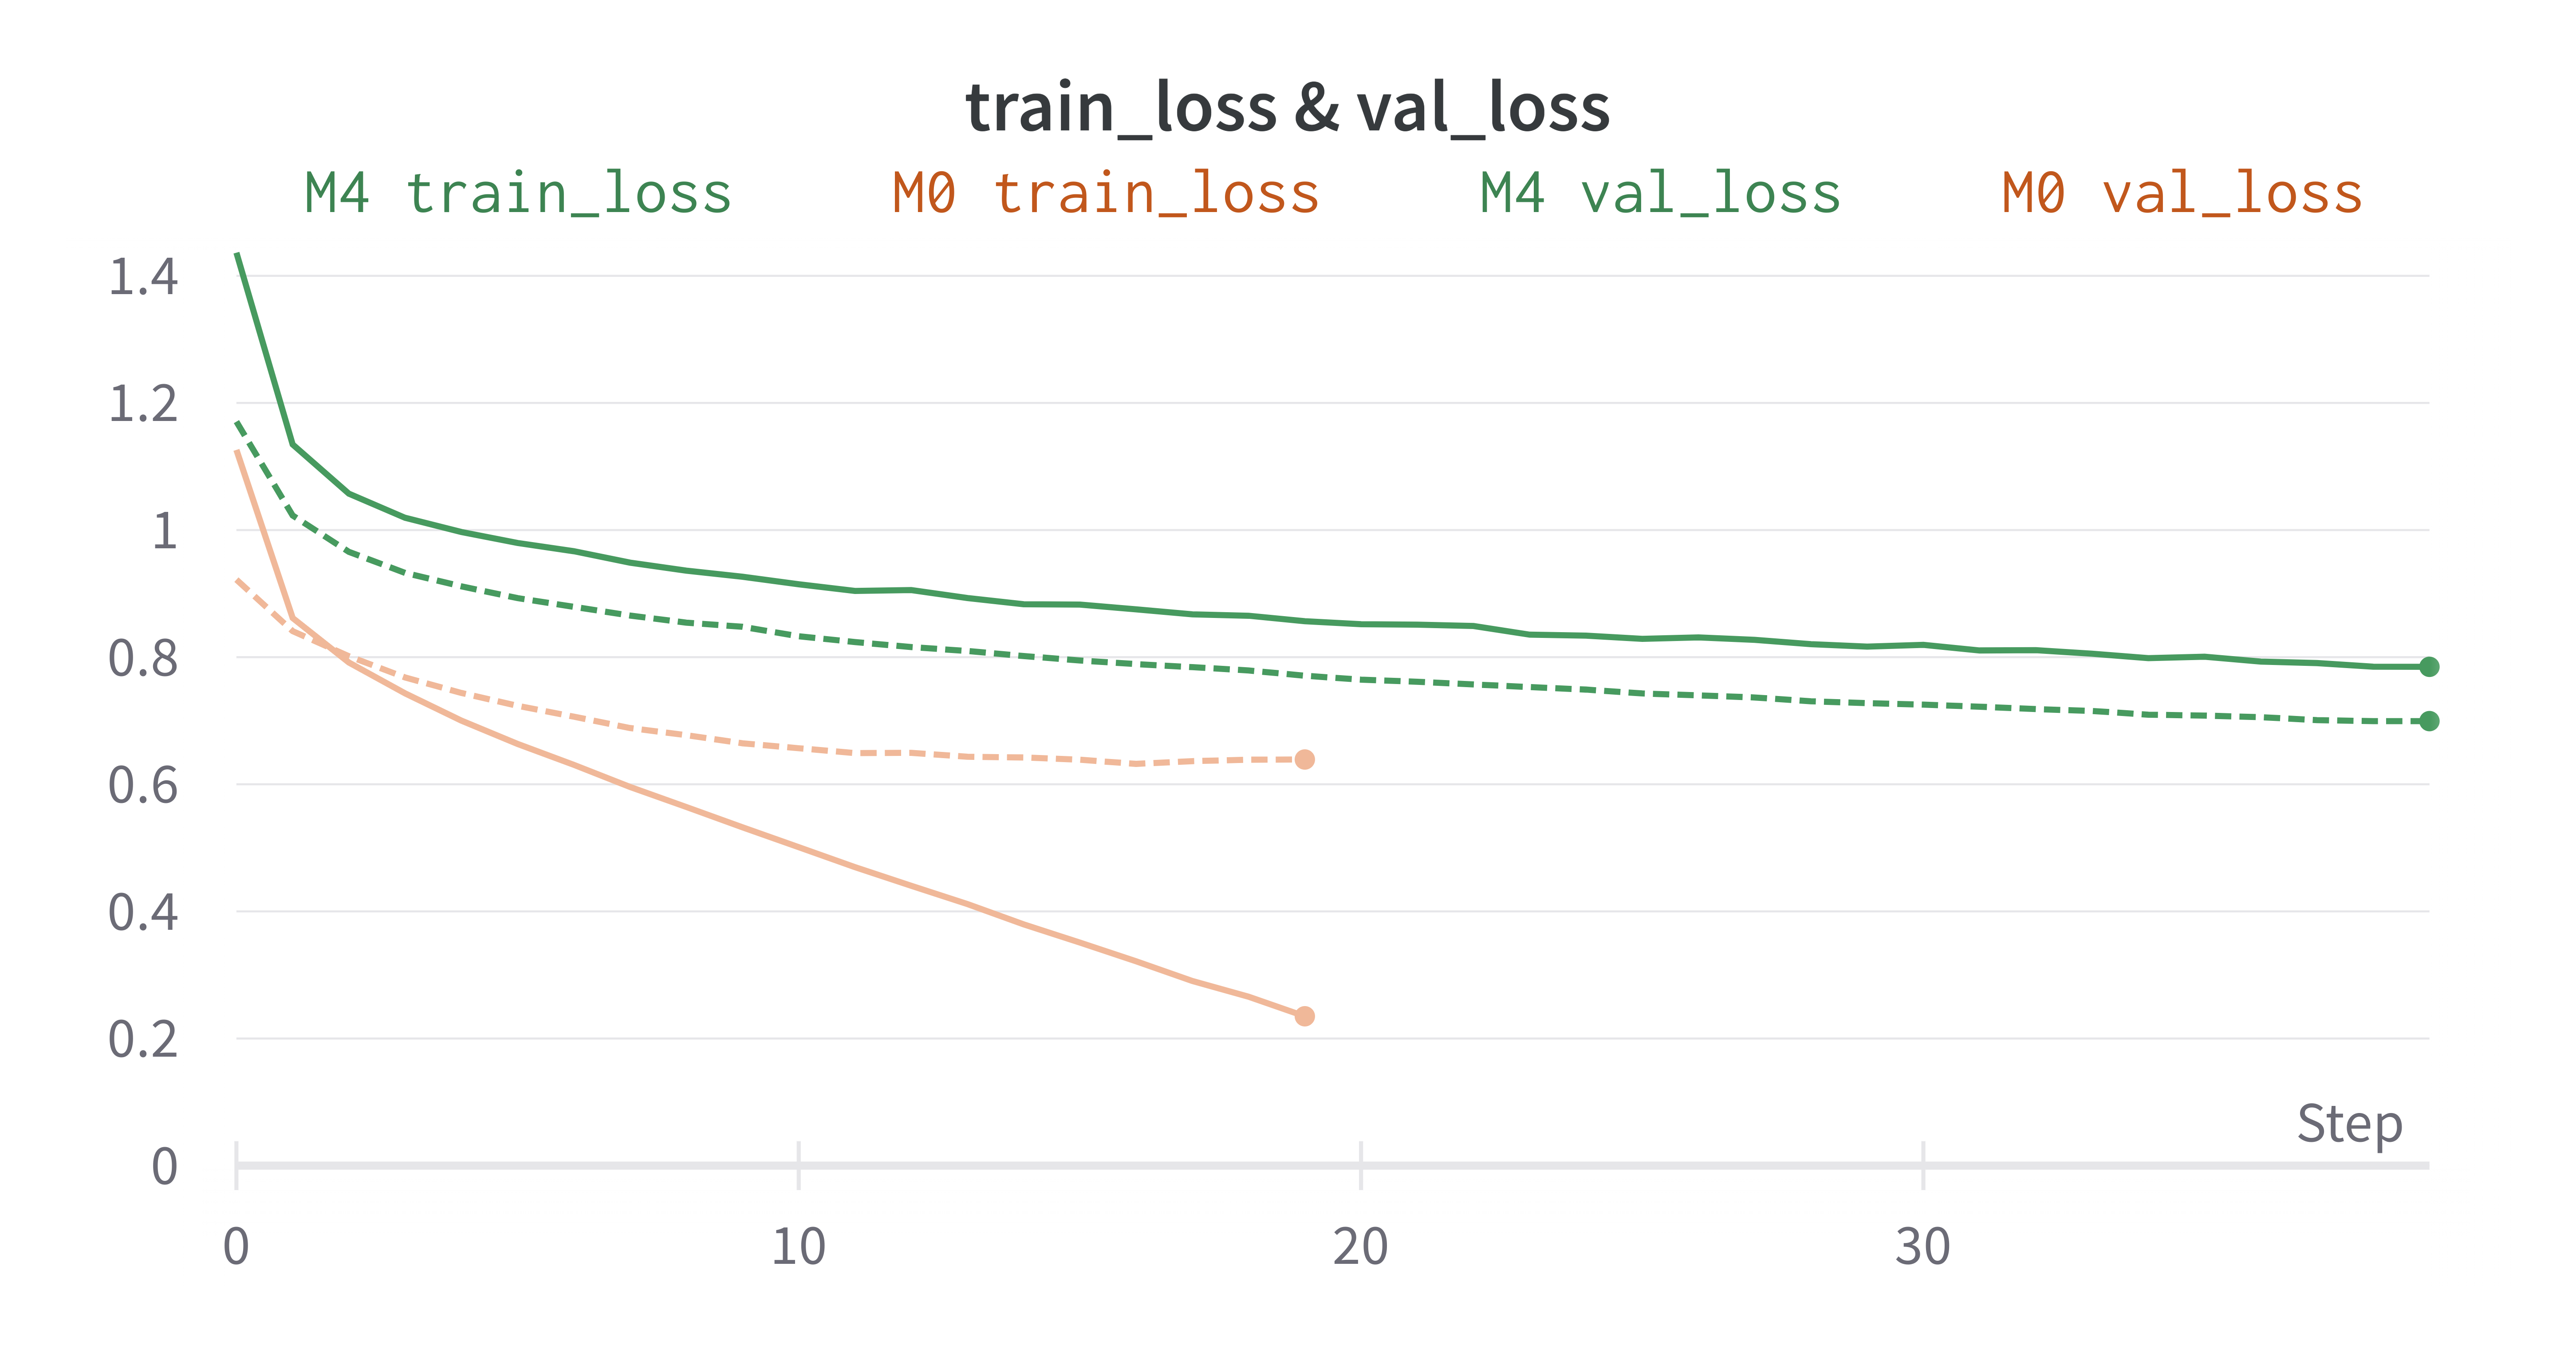
\includegraphics[width=\textwidth]{imatges/results/LossM0M4.png}
  \caption[M0 vs. M4, Loss Train and Validation Curves]{\textit{M0 vs. M4, Loss Train and Validation Curves. }}
  {\label{fig:lossm0m4}}
\end{figure}

\begin{figure}[H]
  \centering
  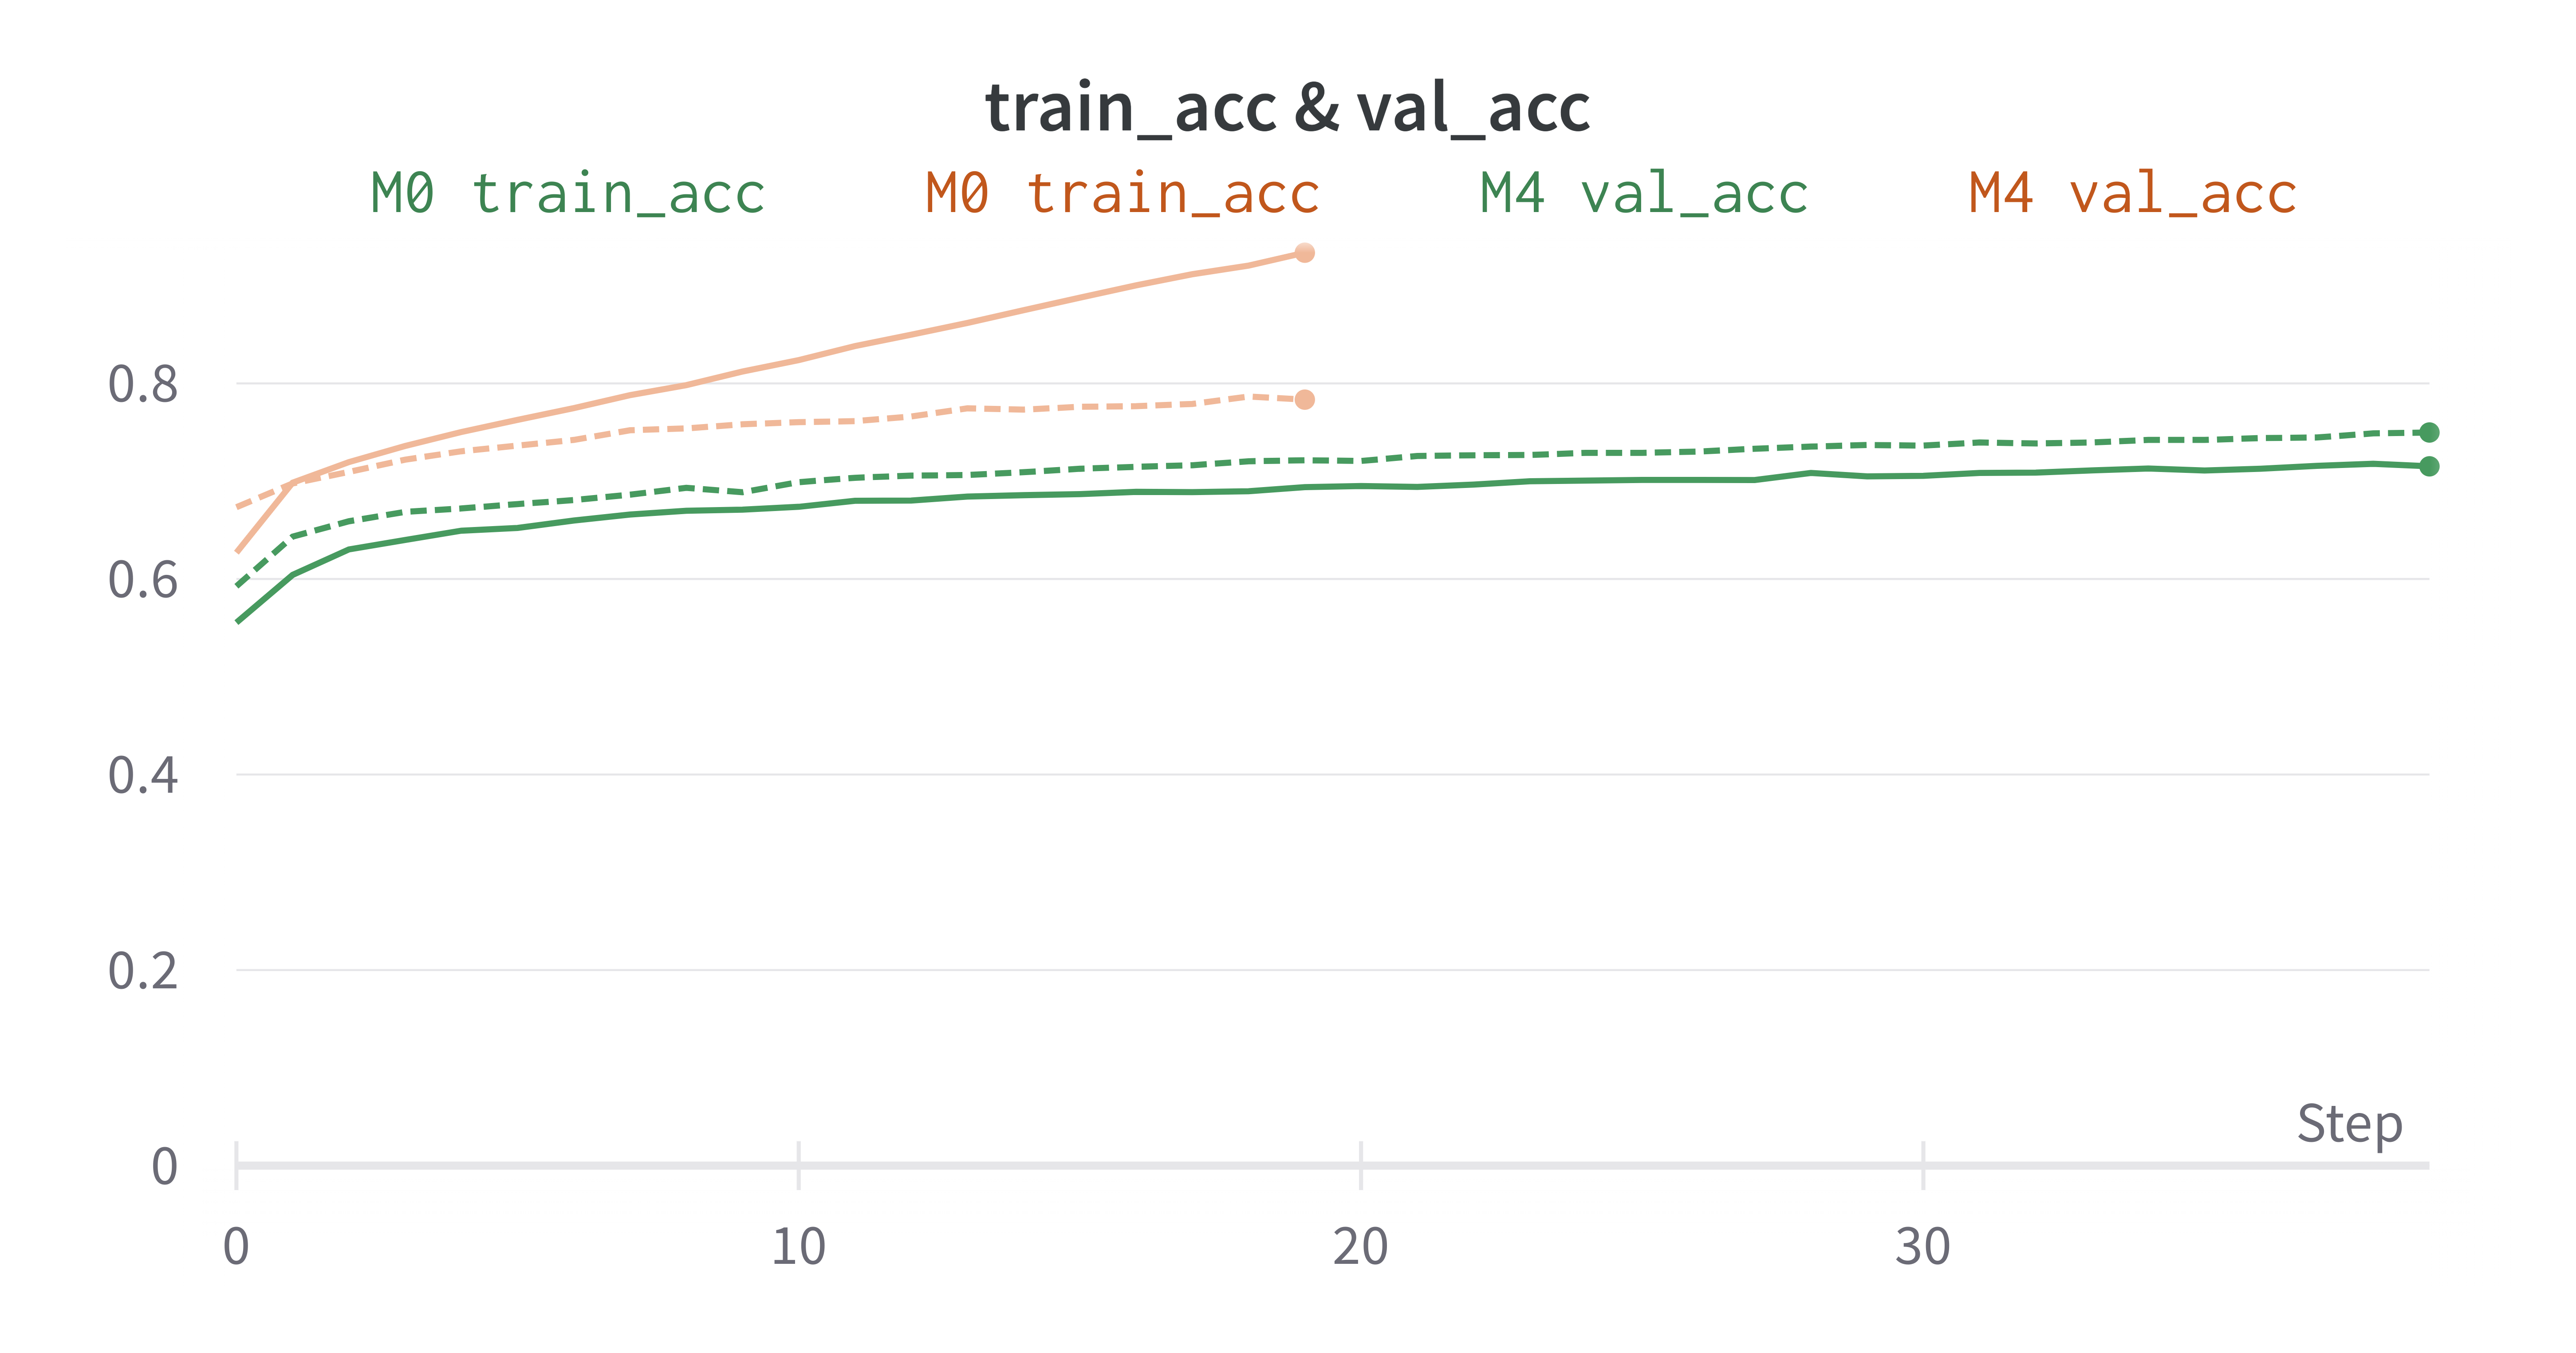
\includegraphics[width=\textwidth]{imatges/results/AccM0M4.png}
  \caption[M0 vs. M4, Acc Train and Validation Curves]{\textit{M0 vs. M4, Acc Train and Validation Curves. }}
\end{figure}

\newpage


\subsection{M1 against M5}

\begin{figure}[H]
  \centering
  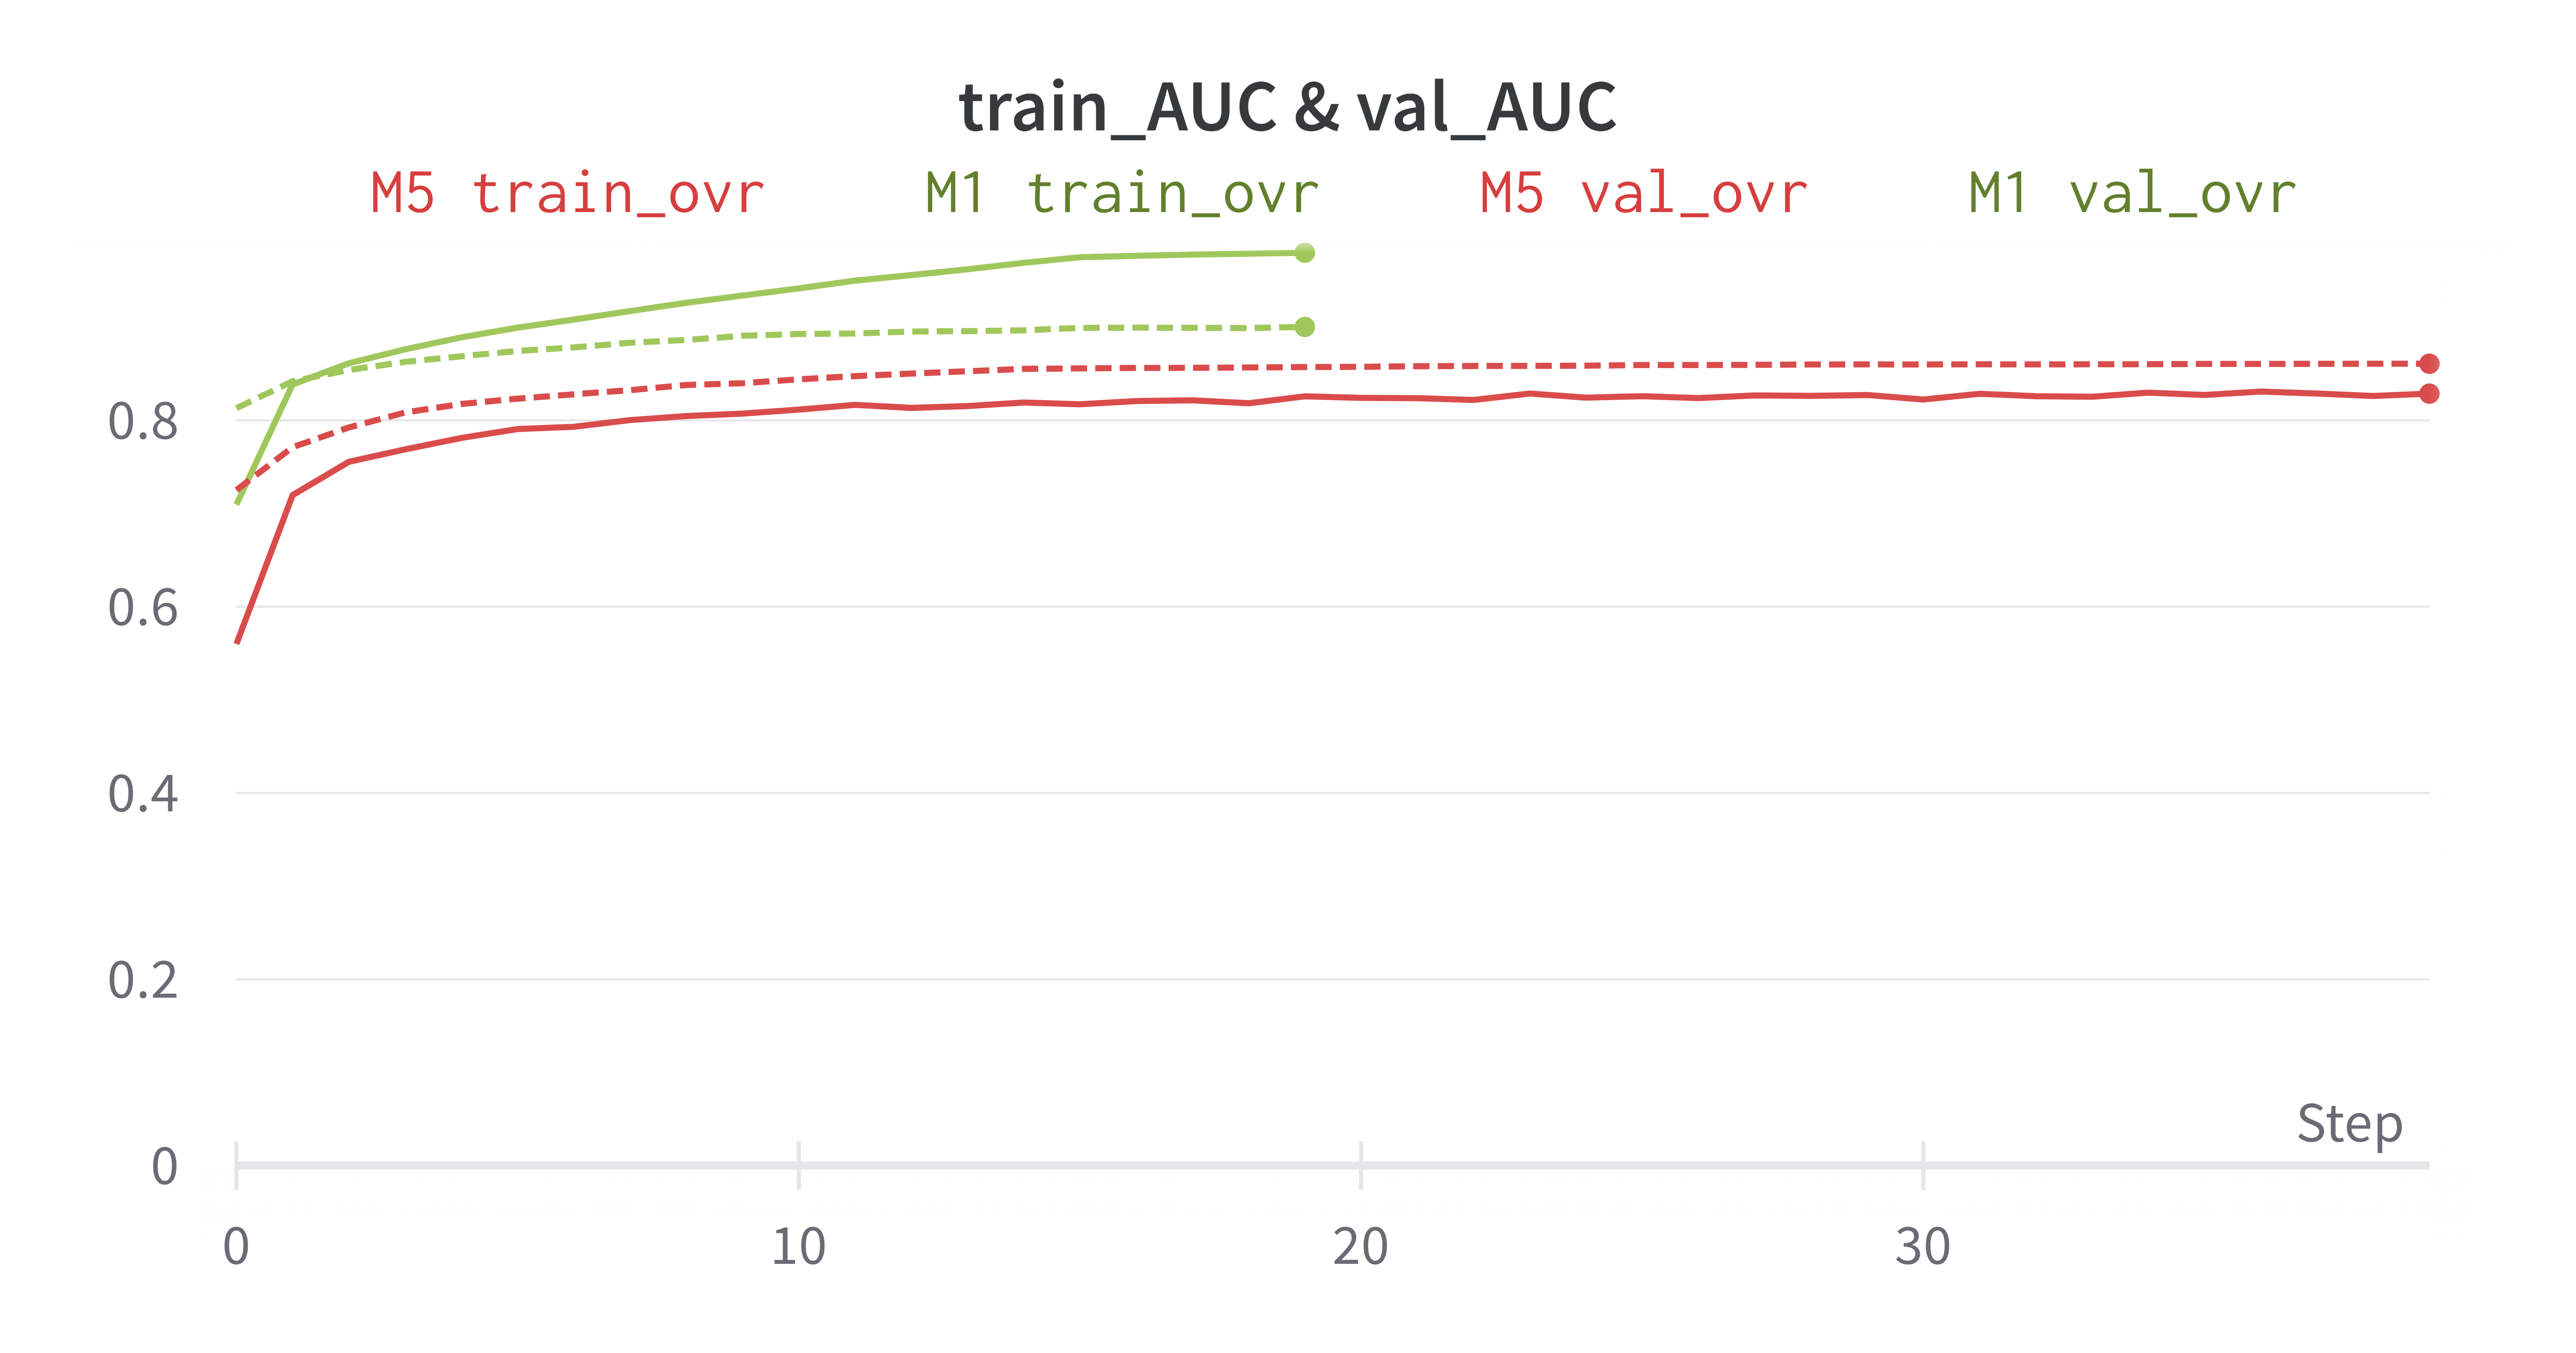
\includegraphics[width=\textwidth]{imatges/results/AUCM1M5.png}
  \caption[M1 vs. M5, AUC Train and Validation Curves]{\textit{M1 vs. M5, AUC Train and Validation Curves. }}
\end{figure}


\begin{figure}[H]
  \centering
  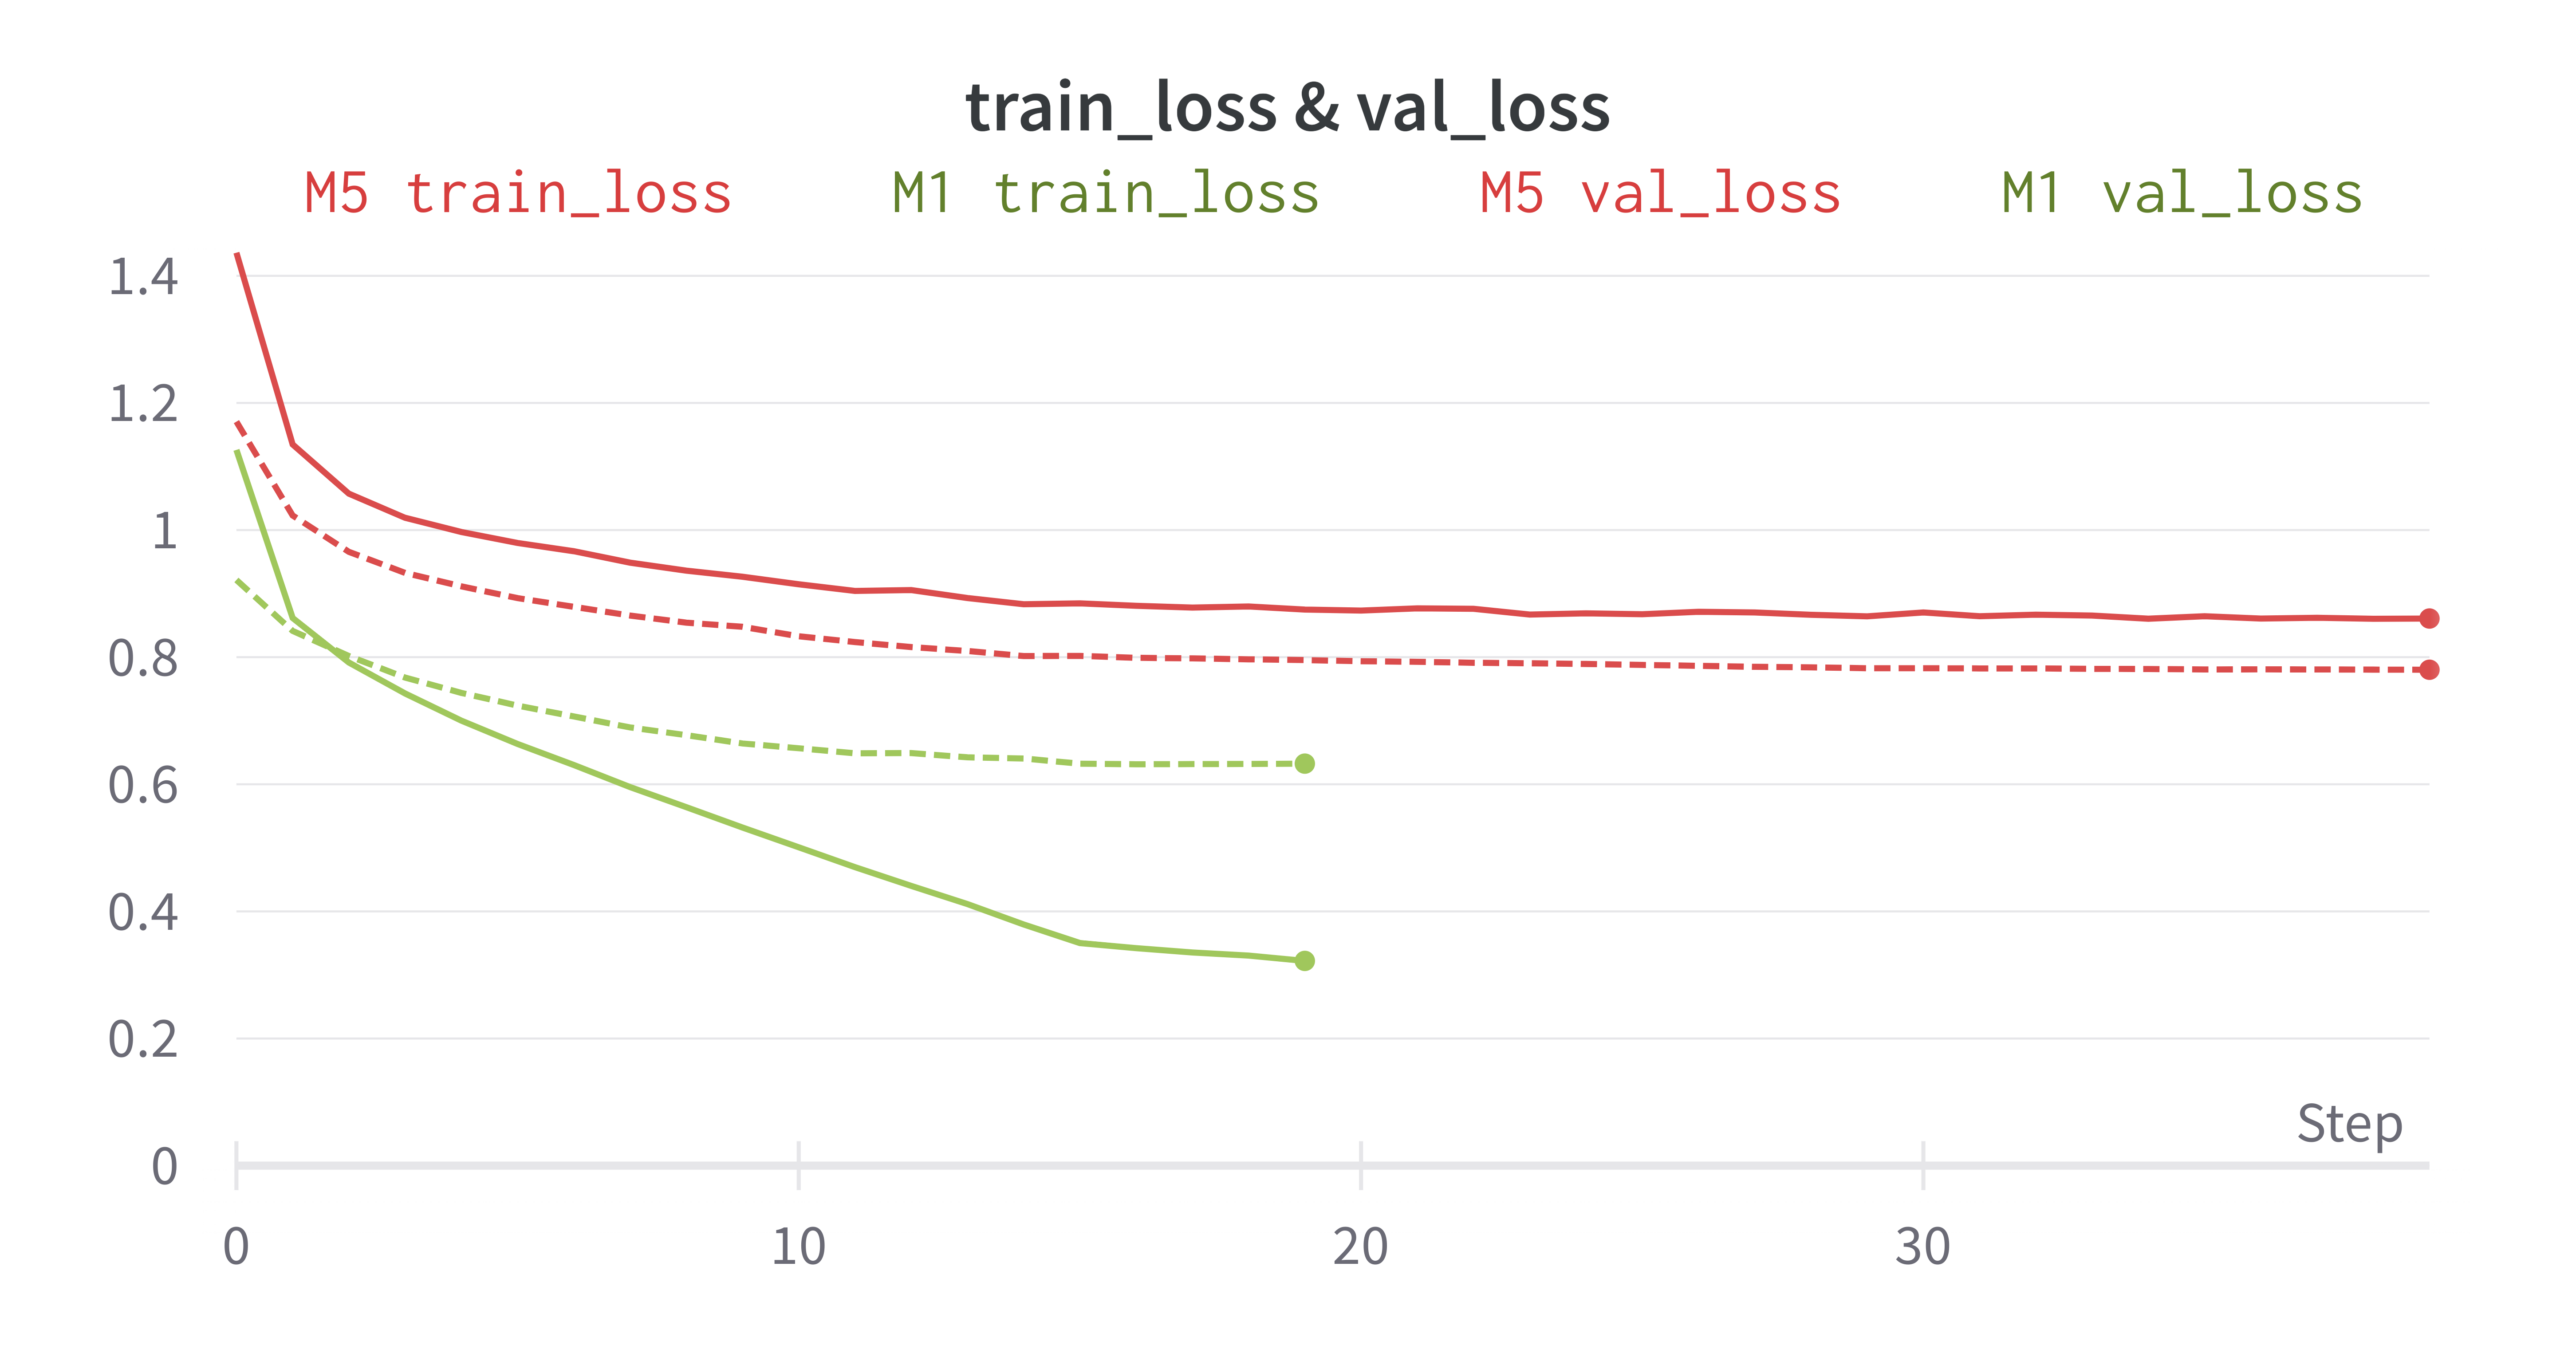
\includegraphics[width=\textwidth]{imatges/results/LossM1M5.png}
  \caption[M1 vs. M5, Loss Train and Validation Curves]{\textit{M1 vs. M5, Loss Train and Validation Curves. }}
\end{figure}

\newpage

\begin{figure}[H]
  \centering
  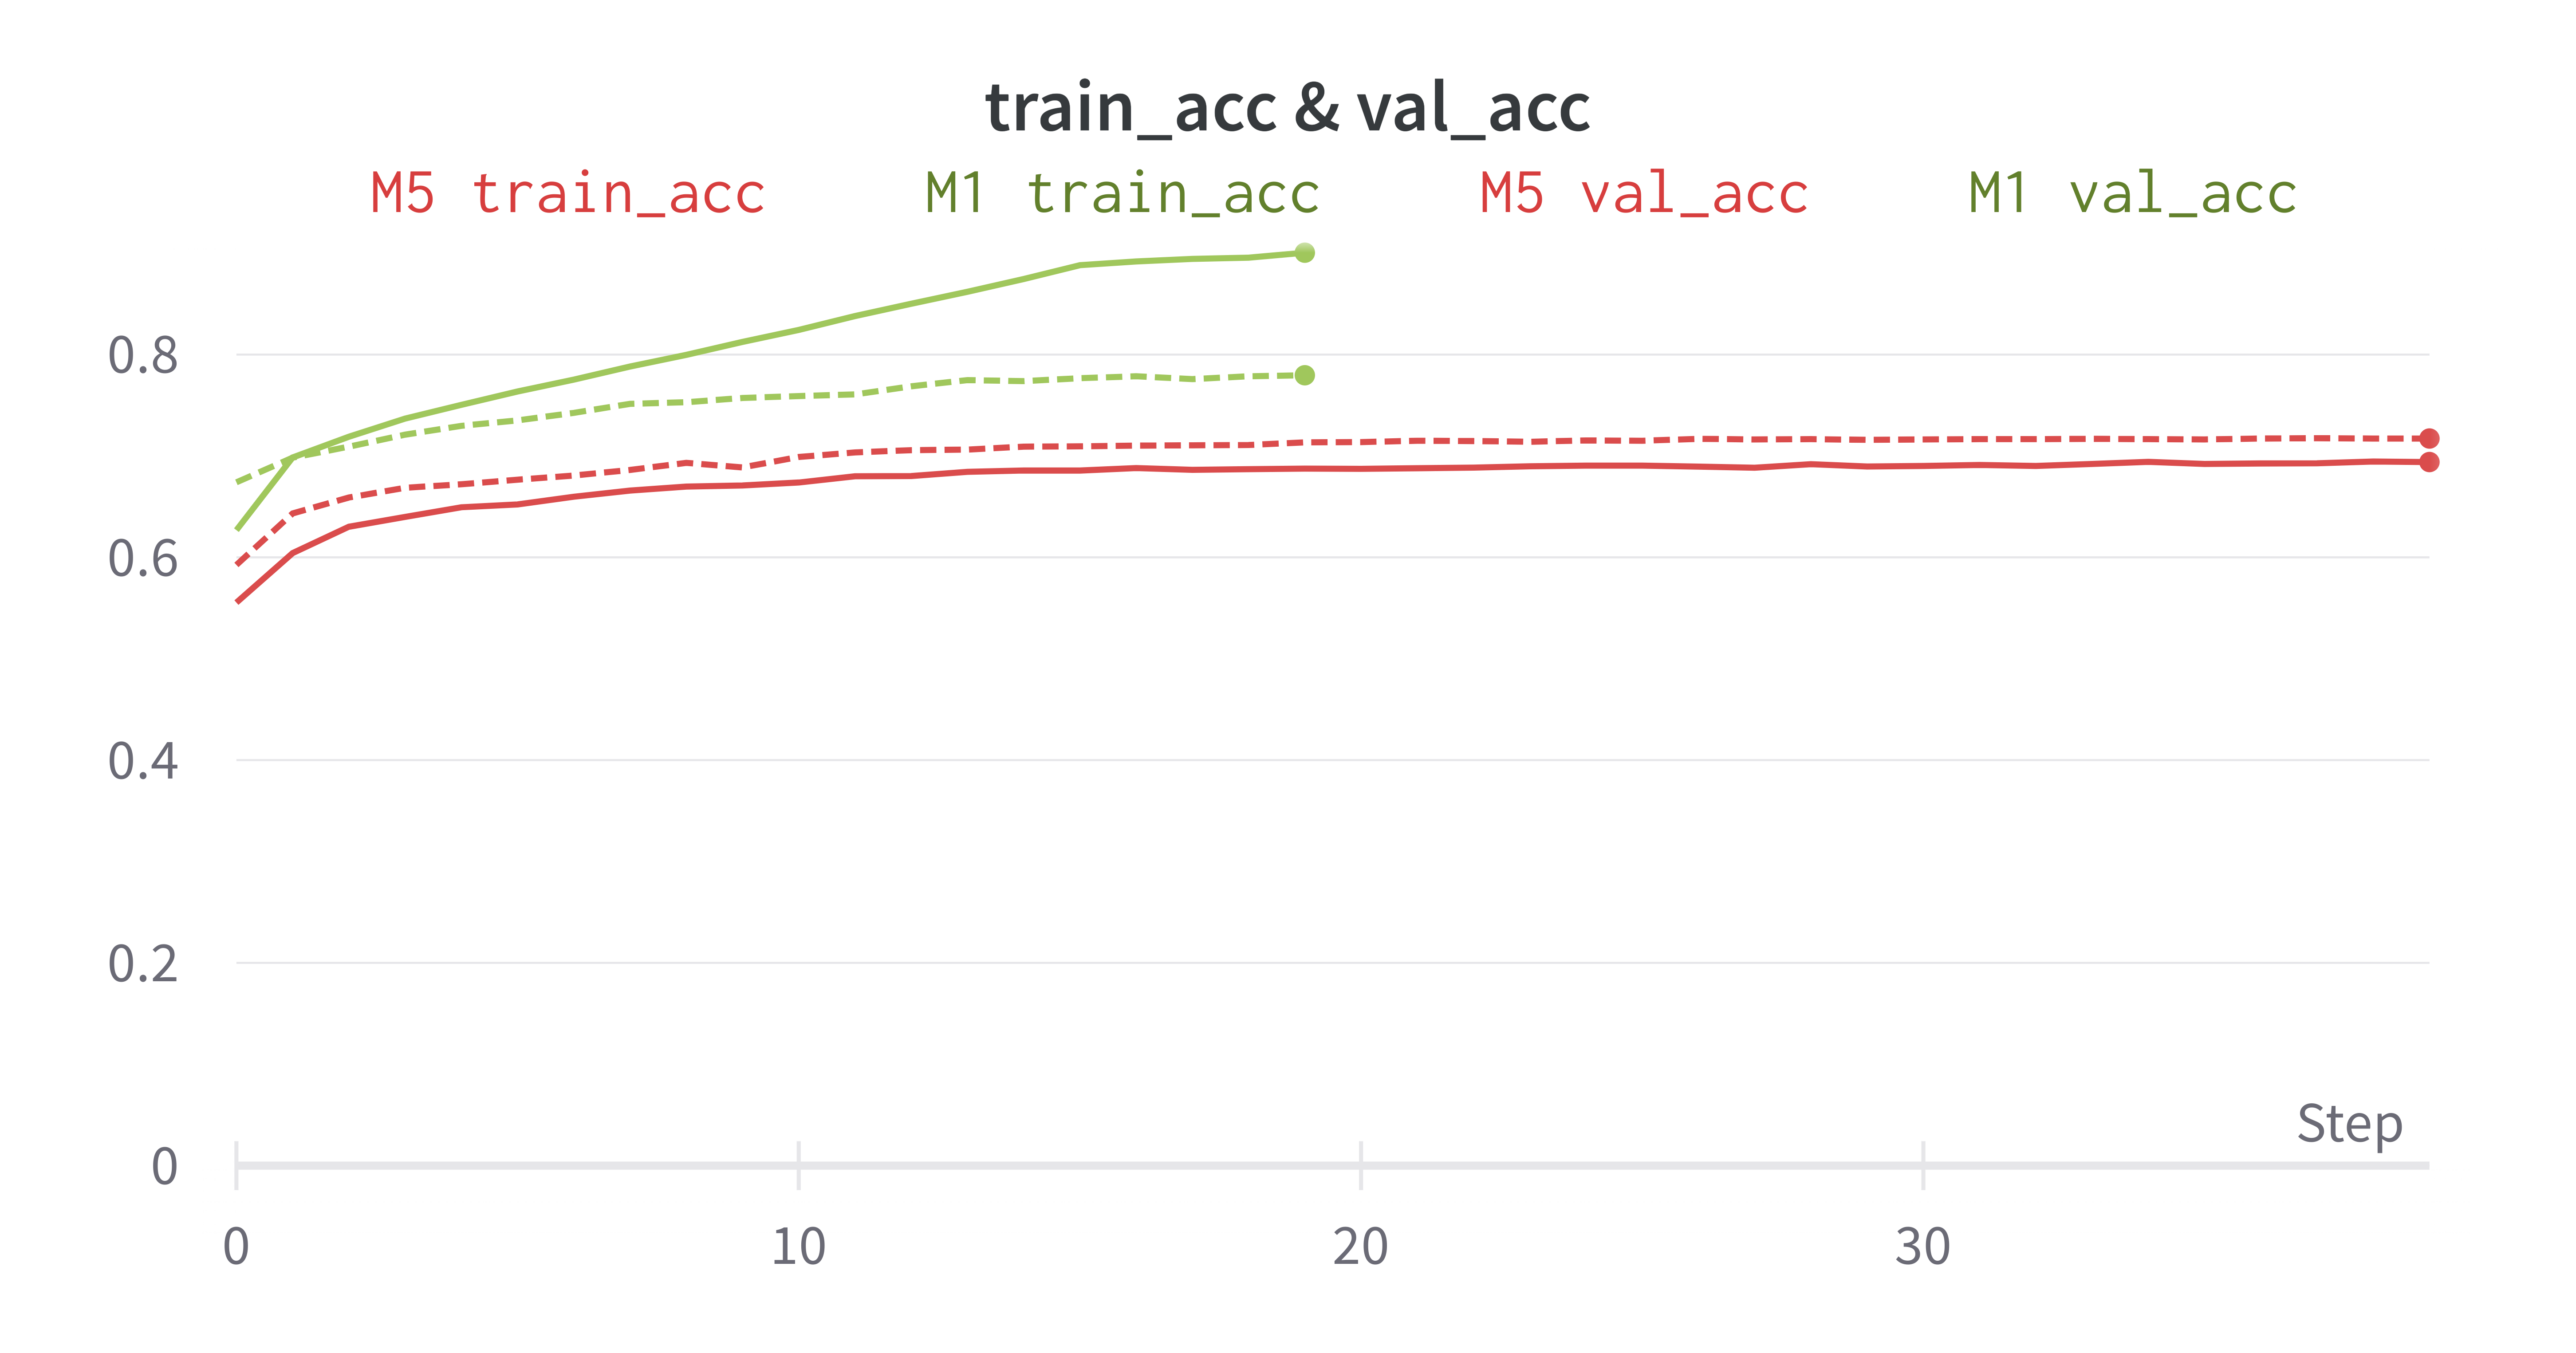
\includegraphics[width=\textwidth]{imatges/results/AccM1M5.png}
  \caption[M1 vs. M5, Acc Train and Validation Curves]{\textit{M1 vs. M5, Acc Train and Validation Curves. }}
\end{figure}


\subsection{M2 against M6}

\begin{figure}[H]
  \centering
  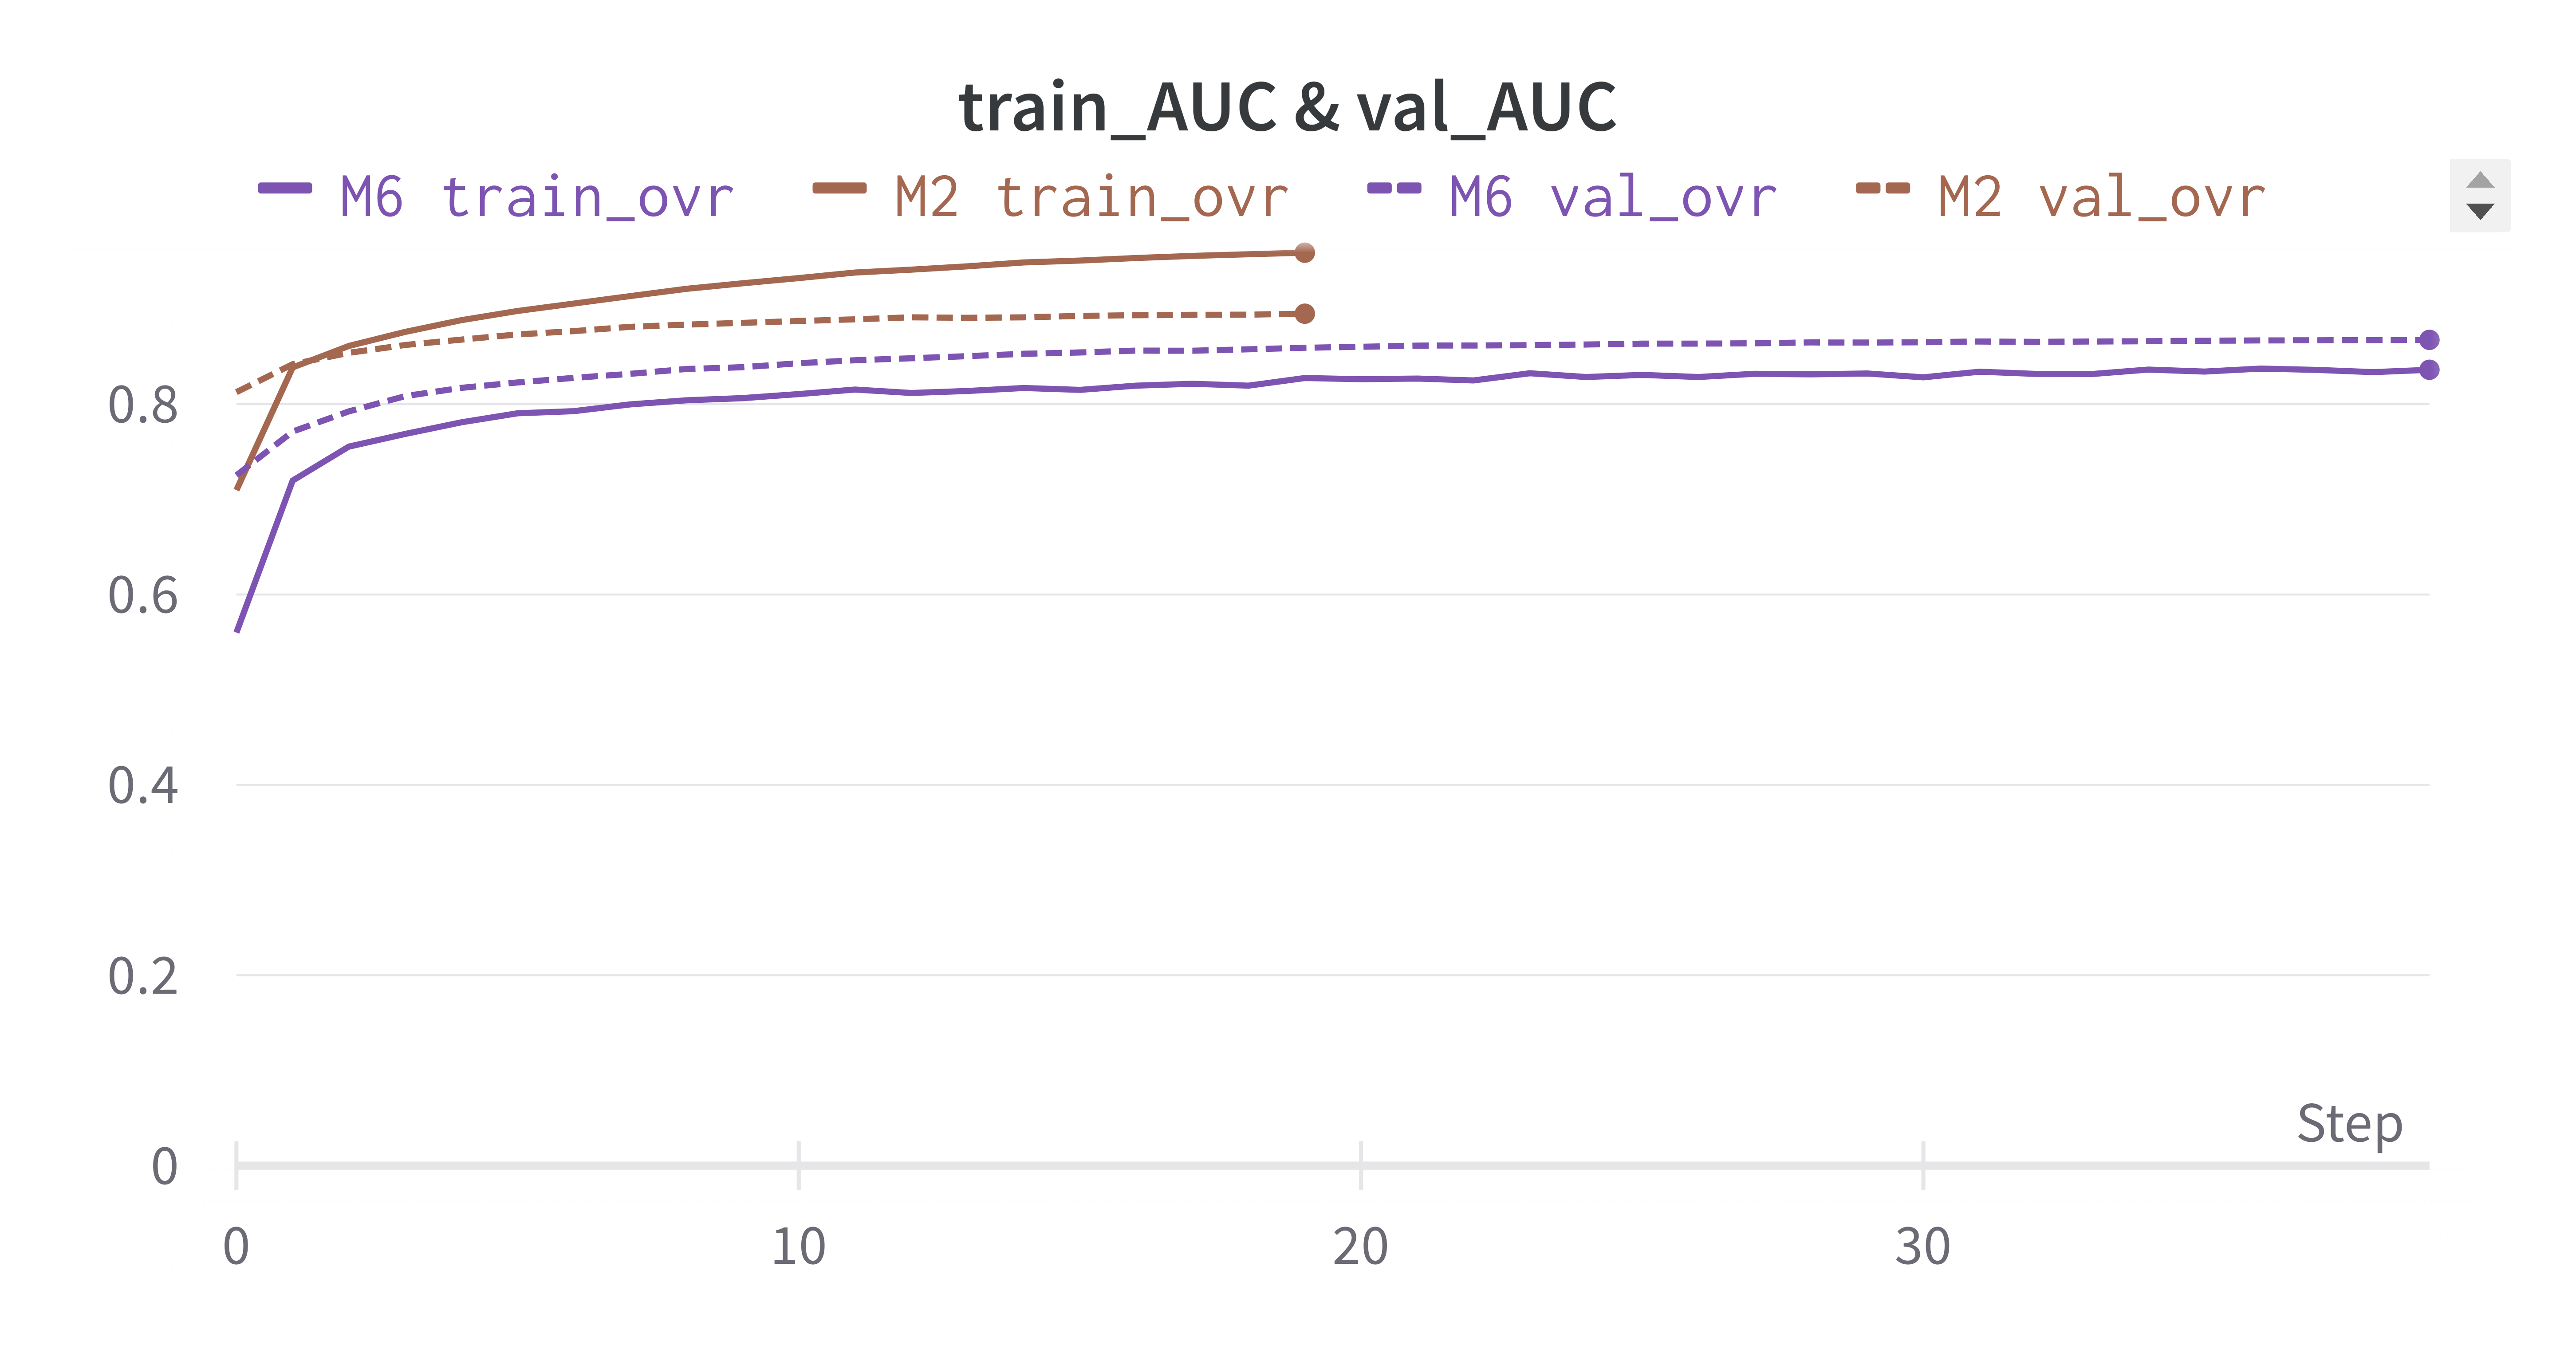
\includegraphics[width=\textwidth]{imatges/results/AUCM2M6.png}
  \caption[M2 vs. M6, AUC Train and Validation Curves]{\textit{M2 vs. M6, AUC Train and Validation Curves. }}
\end{figure}

\newpage

\begin{figure}[H]
  \centering
  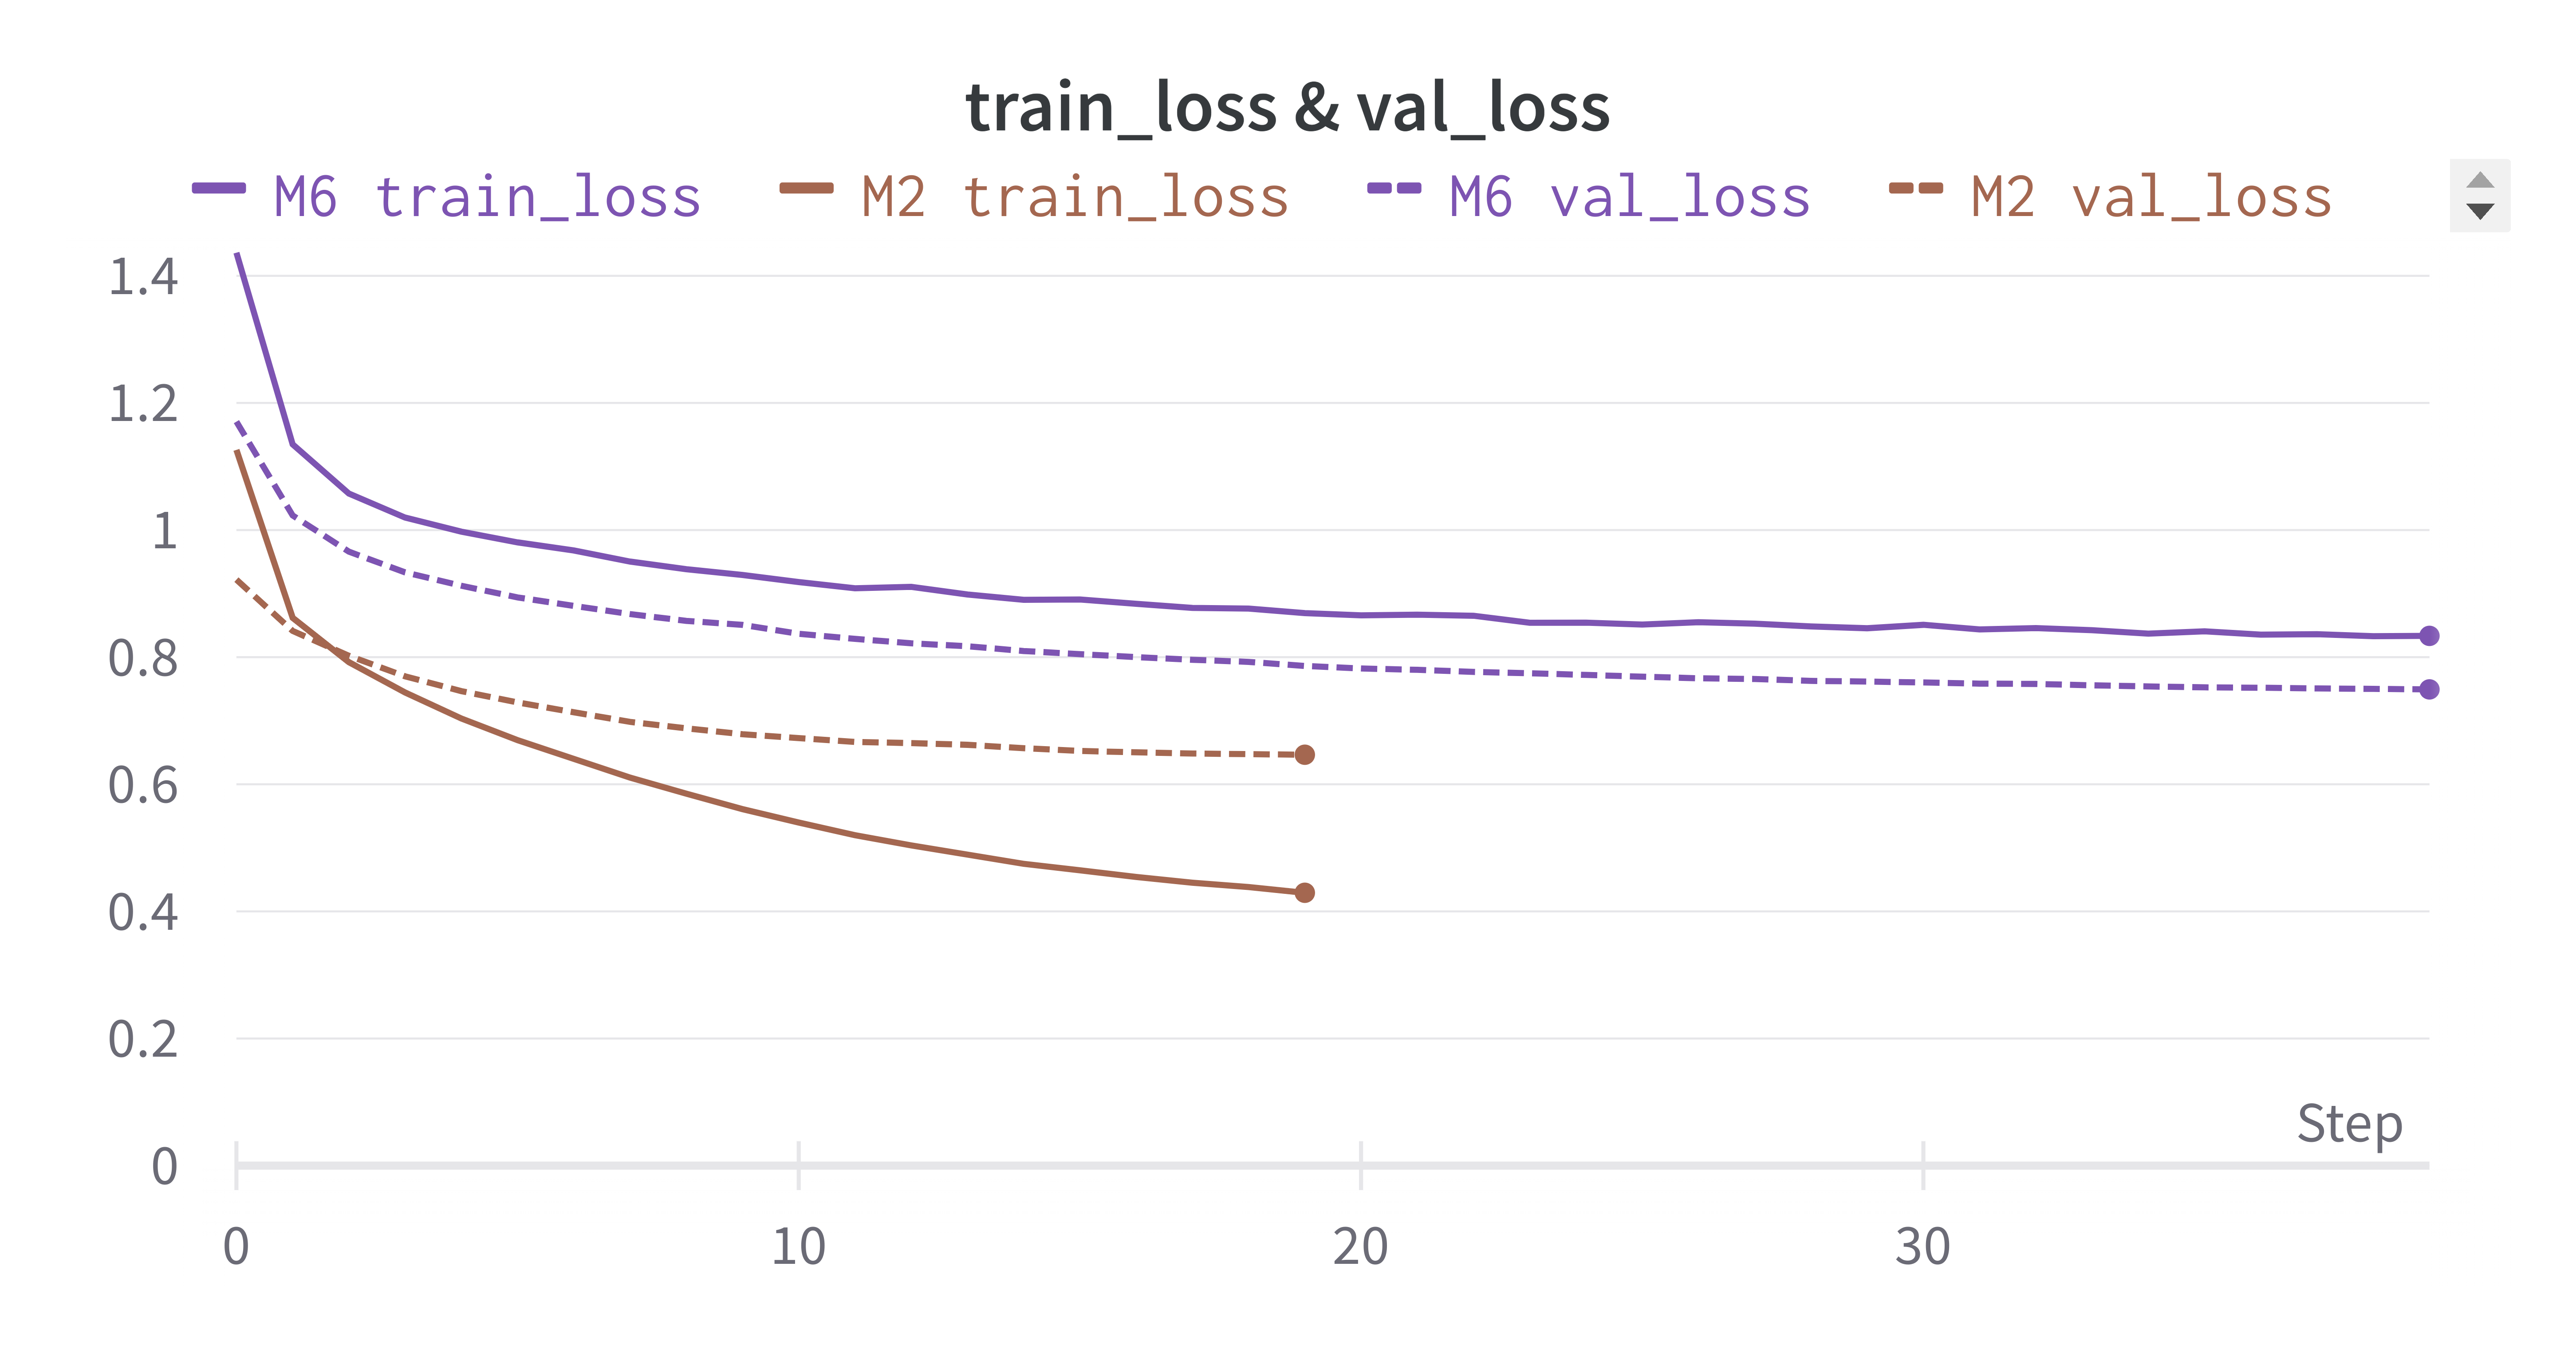
\includegraphics[width=\textwidth]{imatges/results/LossM2M6.png}
  \caption[M2 vs. M6, Loss Train and Validation Curves]{\textit{M2 vs. M6, Loss Train and Validation Curves. }}
\end{figure}


\begin{figure}[H]
  \centering
  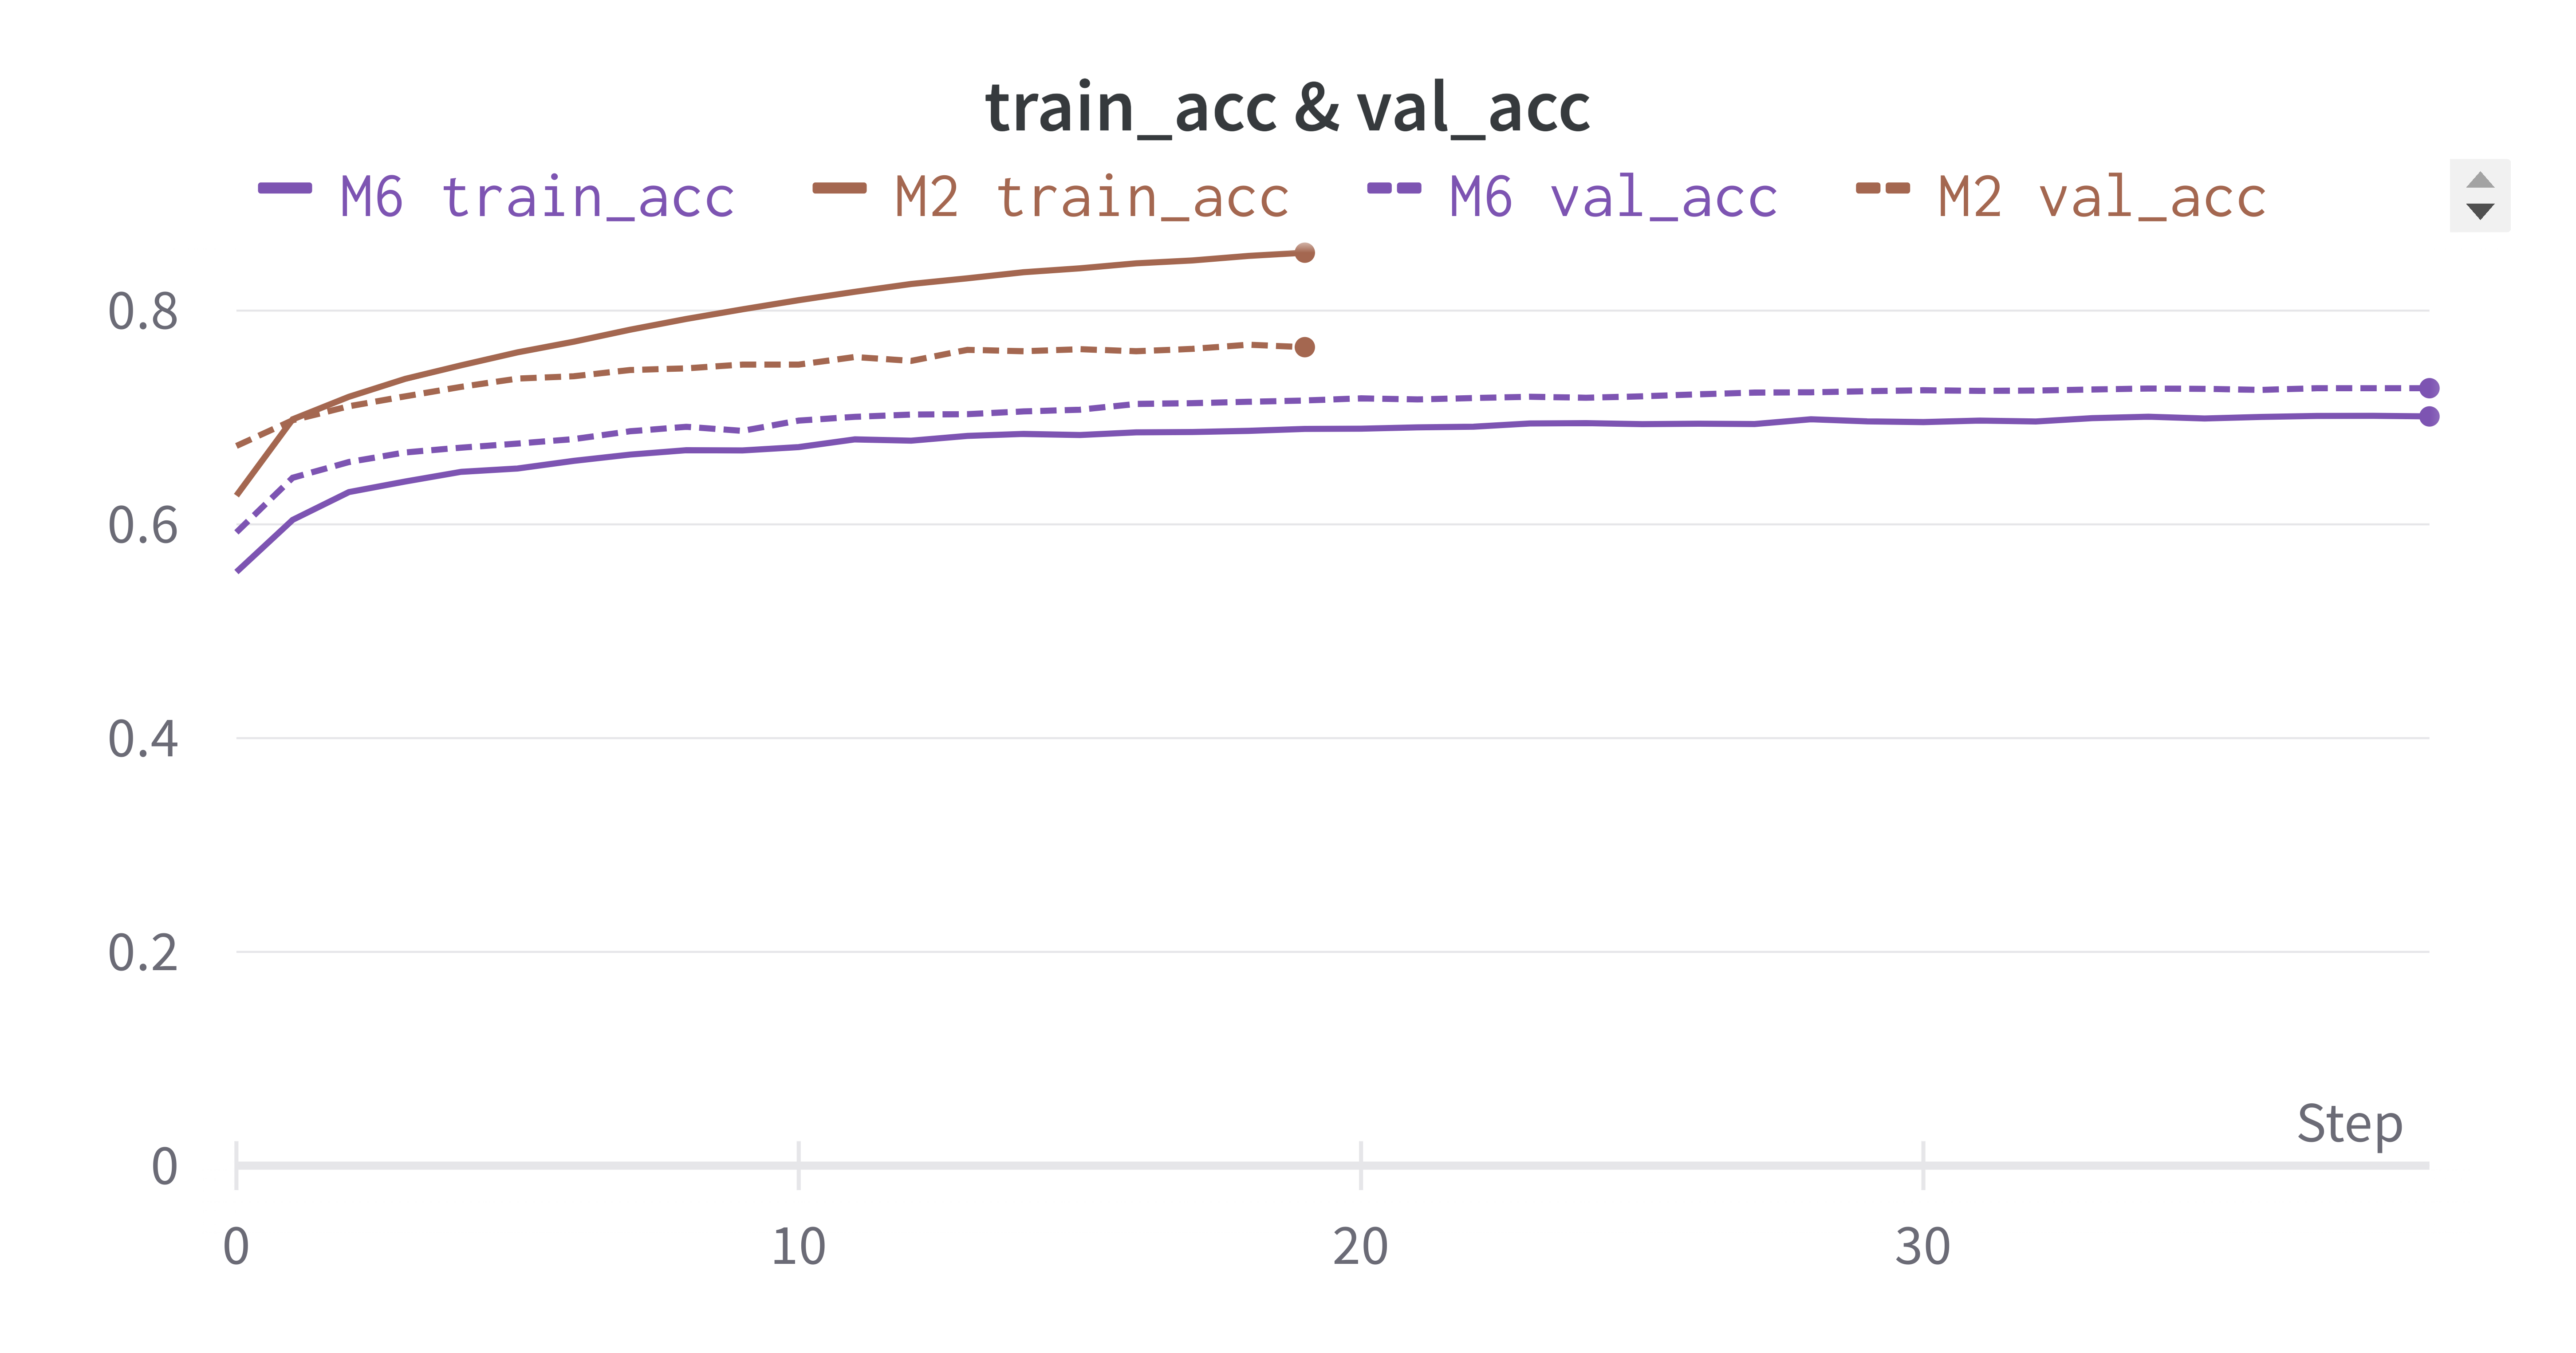
\includegraphics[width=\textwidth]{imatges/results/AccM2M6.png}
  \caption[M2 vs. M6, Acc Train and Validation Curves]{\textit{M2 vs. M6, Acc Train and Validation Curves. }}
\end{figure}

\newpage

\subsection{M3 against M7}

\begin{figure}[H]
  \centering
  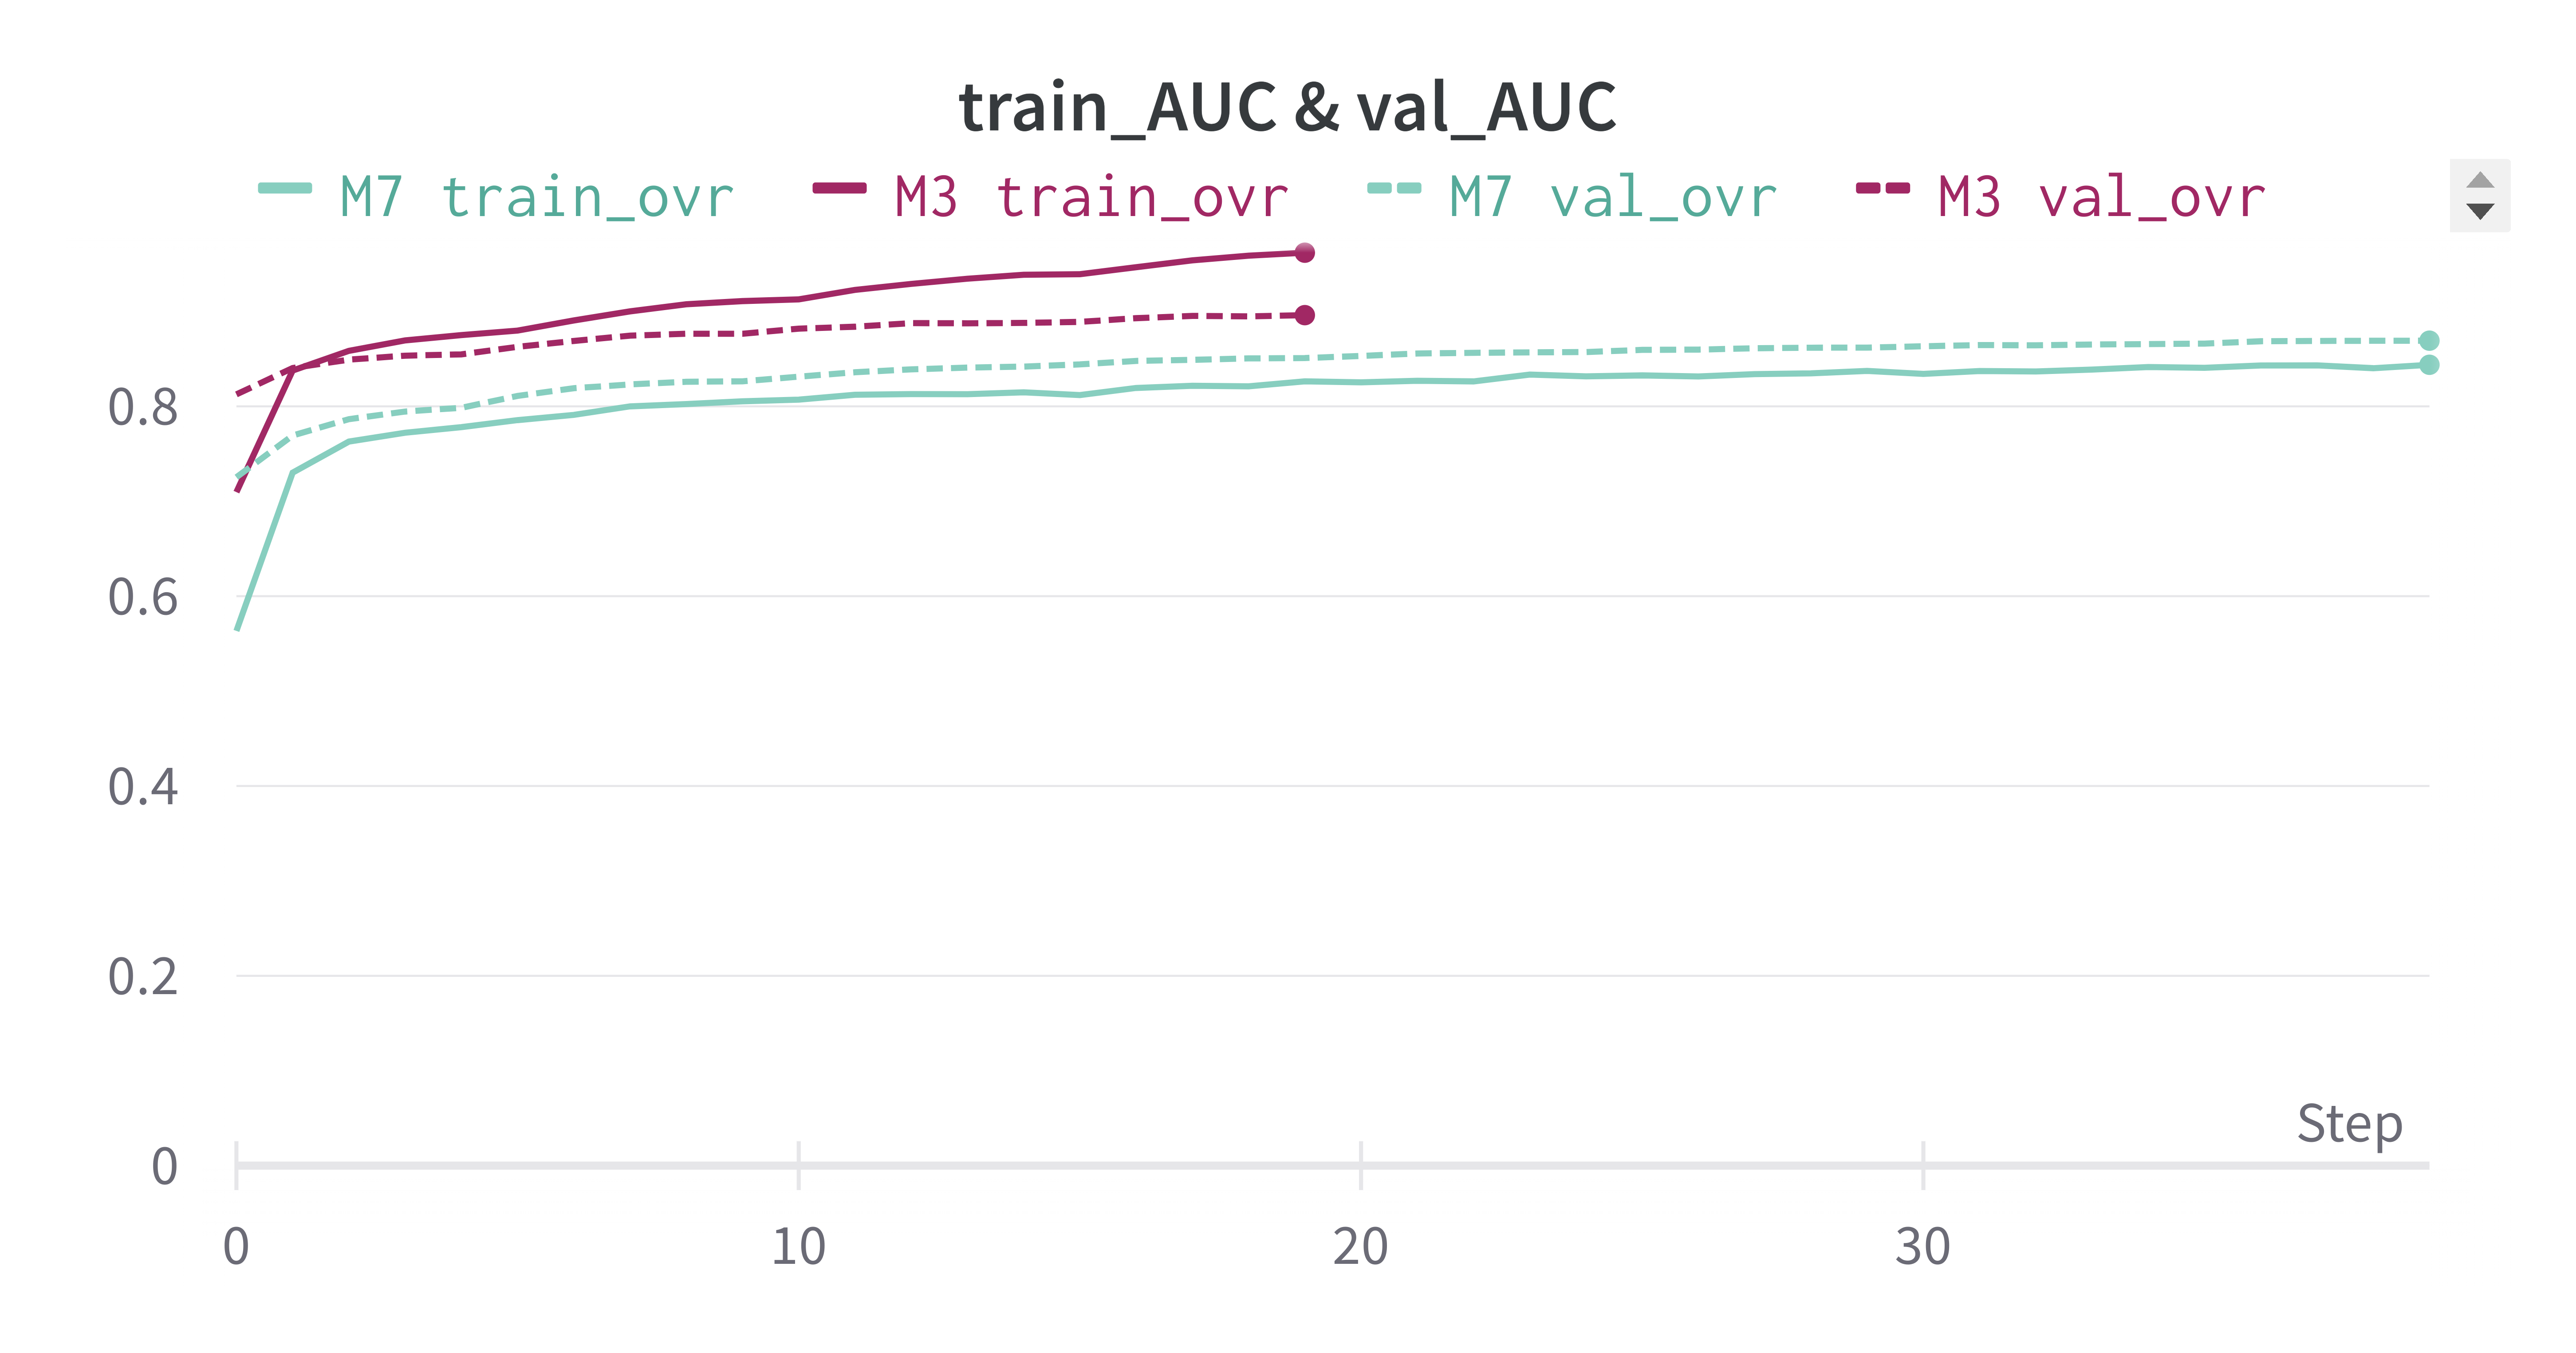
\includegraphics[width=\textwidth]{imatges/results/AUCM3M7.png}
  \caption[M3 vs. M7, AUC Train and Validation Curves]{\textit{M3 vs. M7, AUC Train and Validation Curves. }}
\end{figure}


\begin{figure}[H]
  \centering
  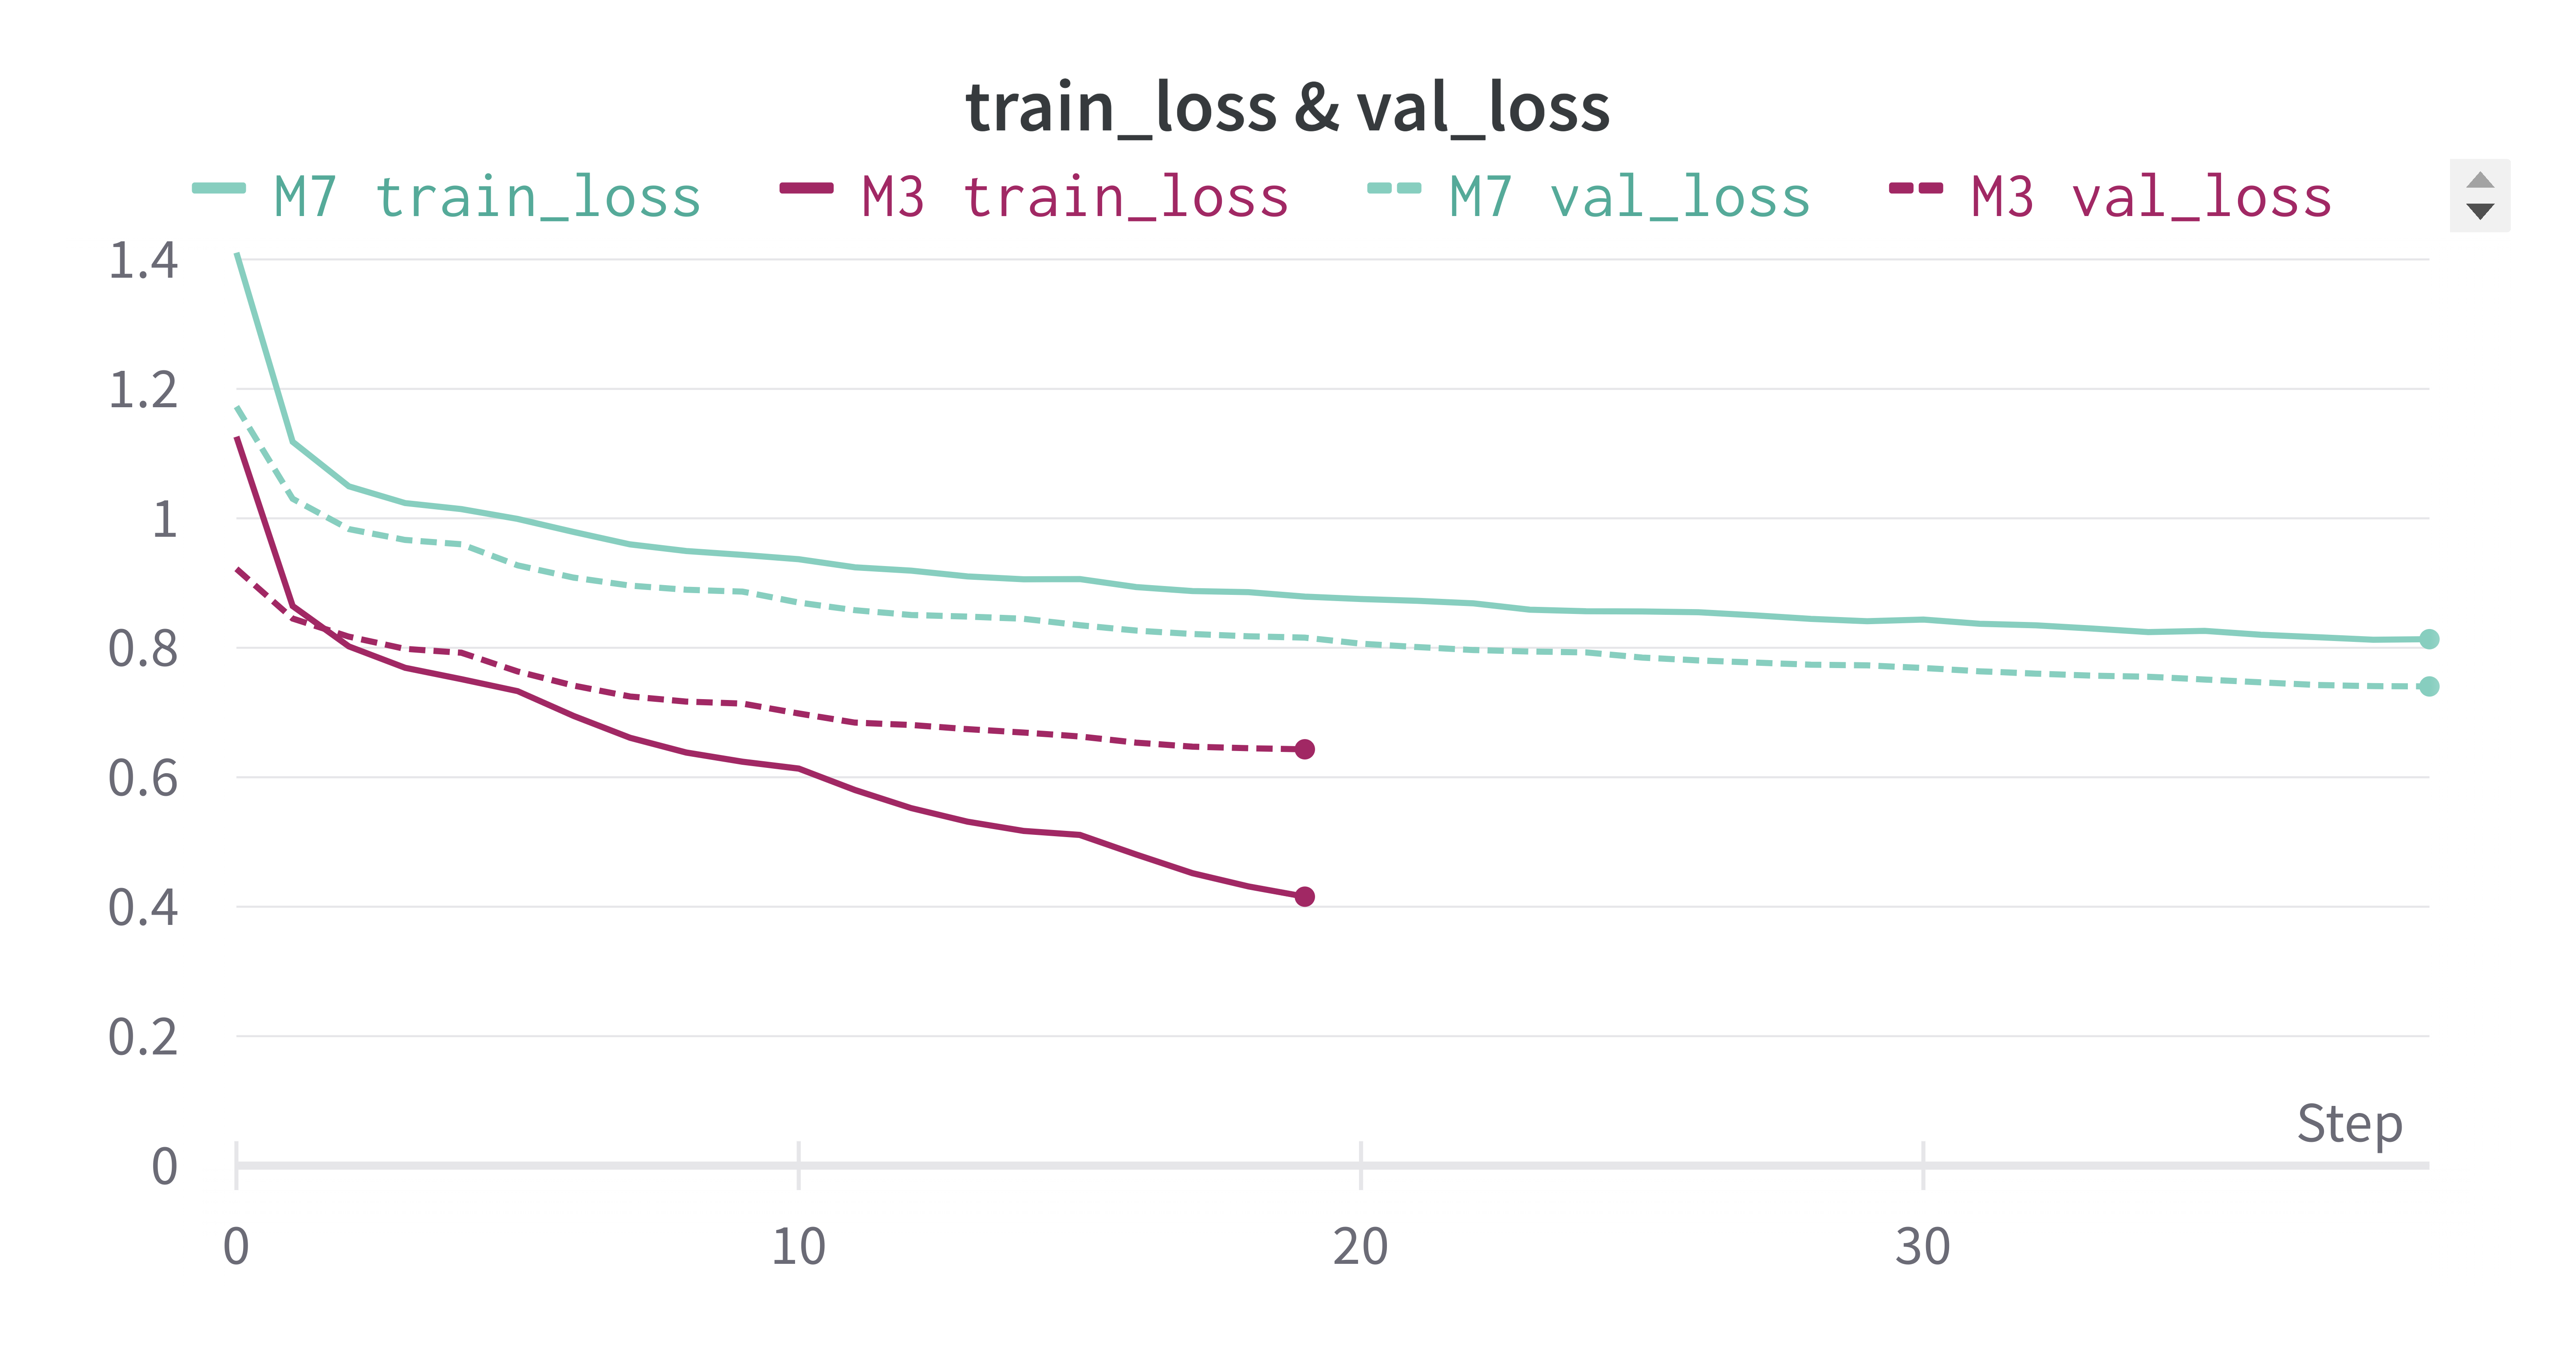
\includegraphics[width=\textwidth]{imatges/results/LossM3M7.png}
  \caption[M3 vs. M7, Loss Train and Validation Curves]{\textit{M3 vs. M7, Loss Train and Validation Curves. }}
\end{figure}

\newpage

\begin{figure}[H]
  \centering
  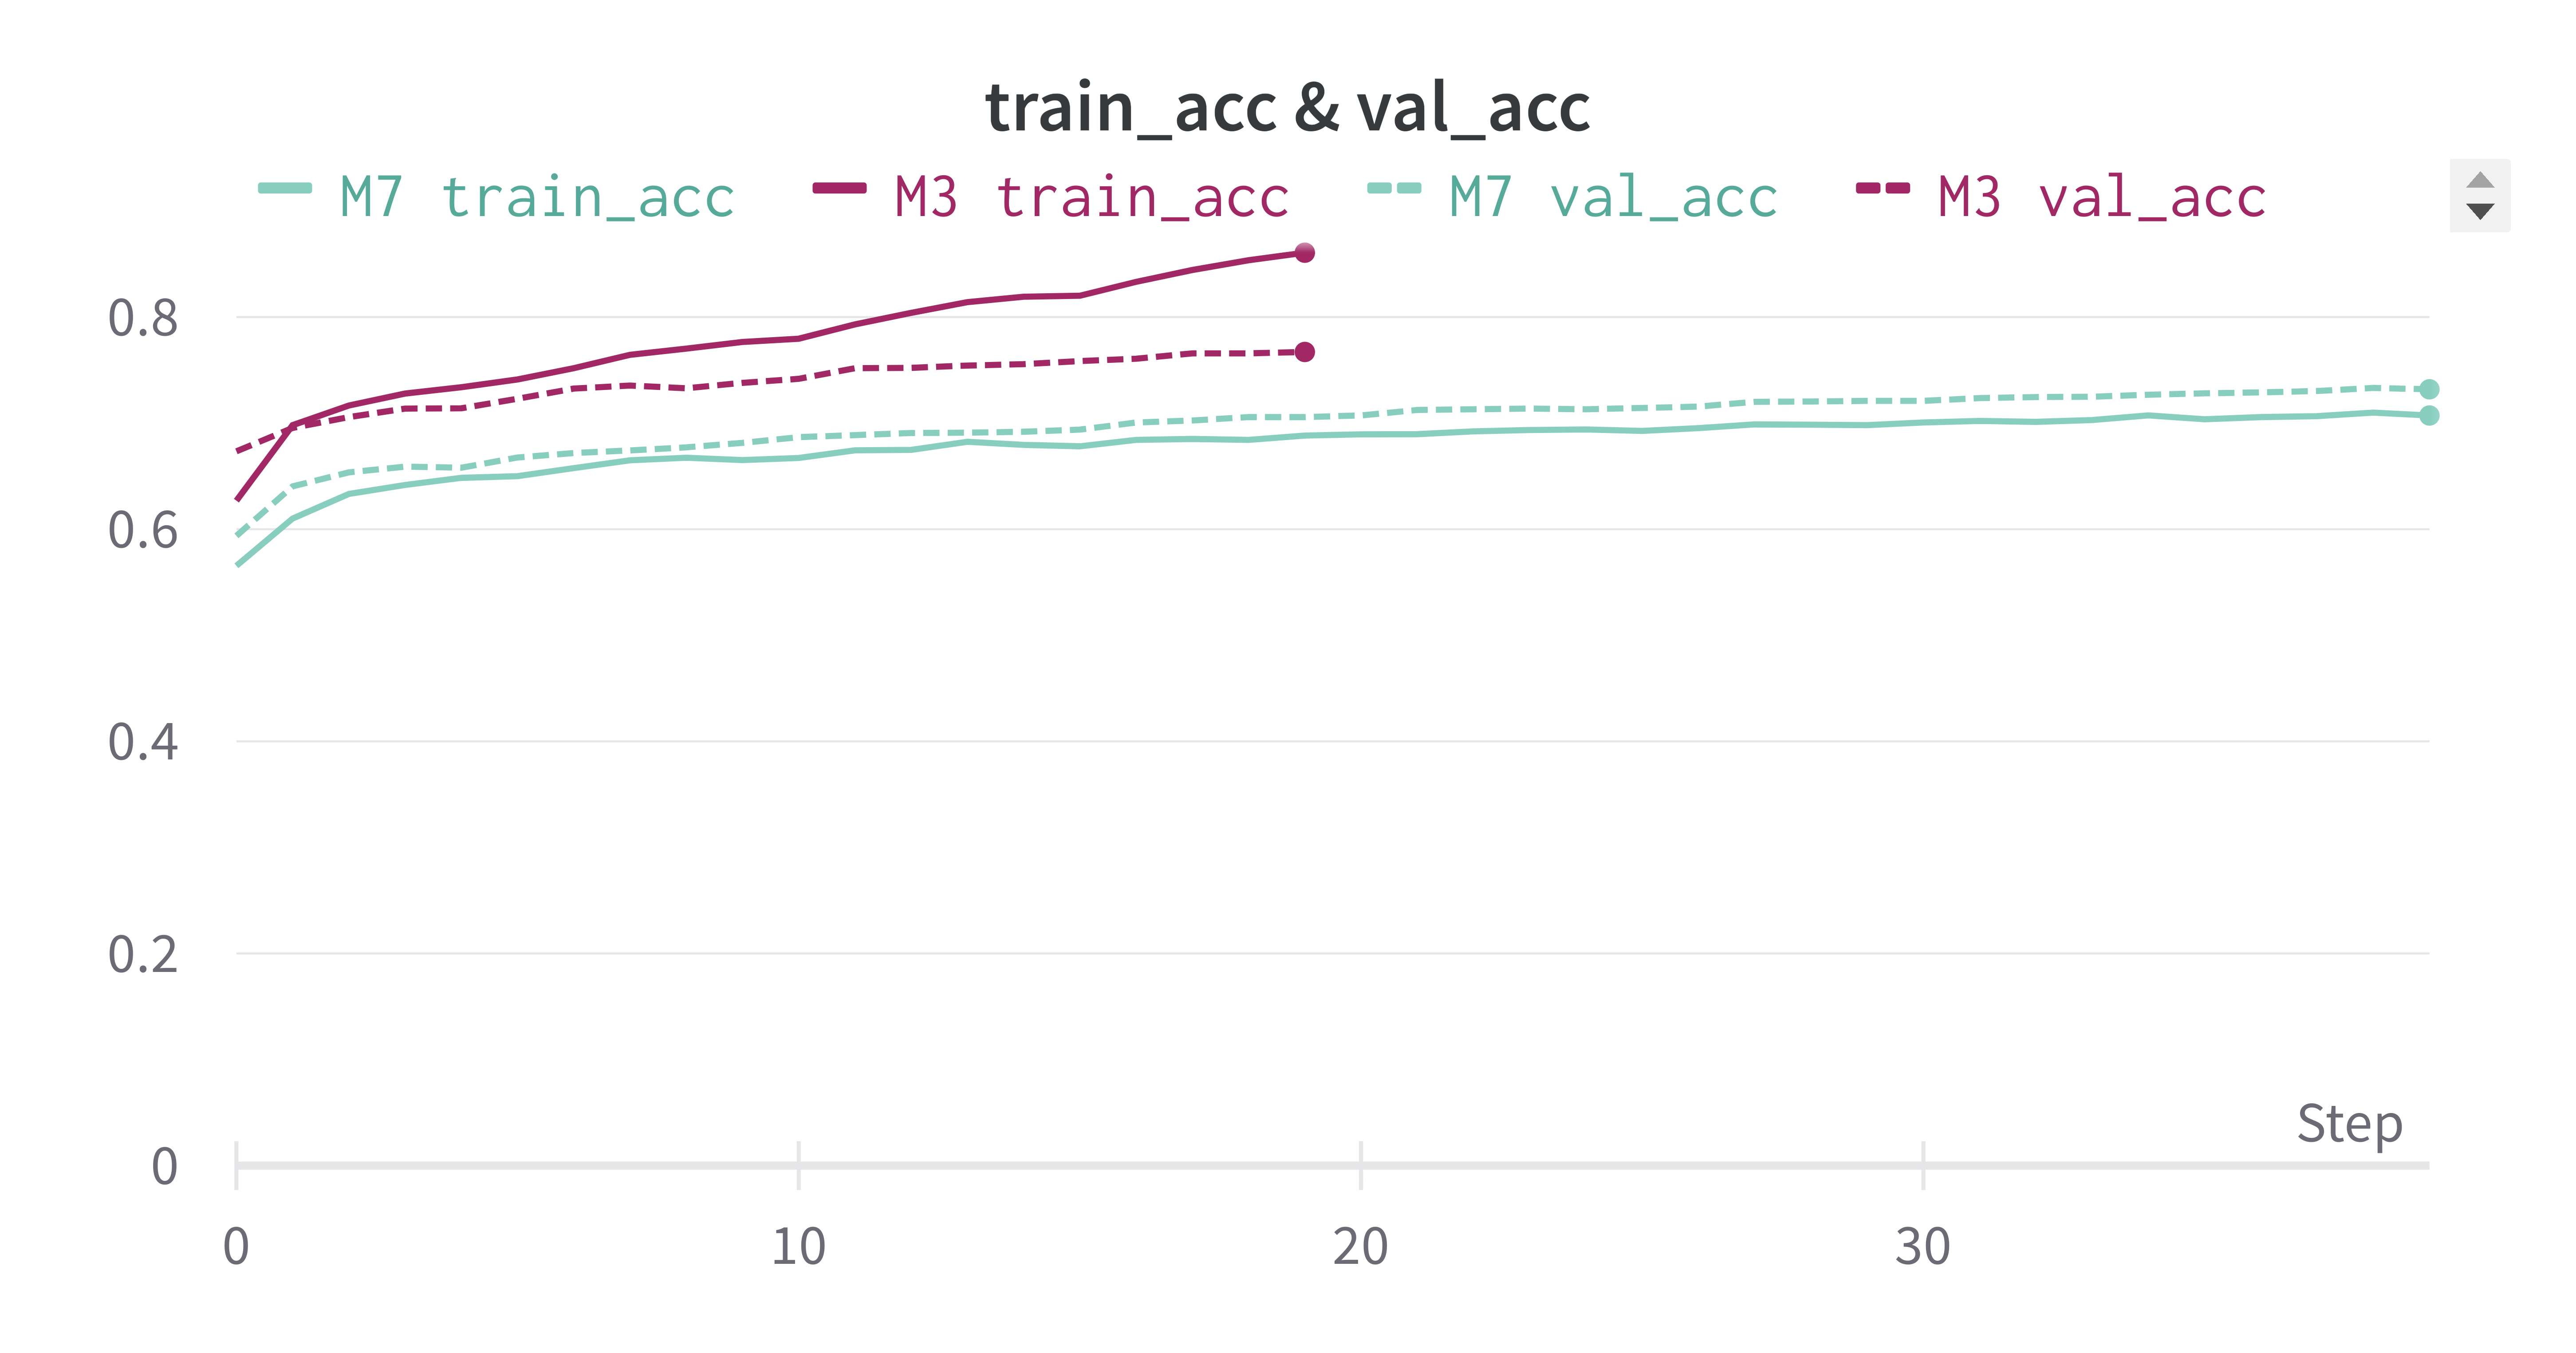
\includegraphics[width=\textwidth]{imatges/results/AccM3M7.png}
  \caption[M3 vs. M7, Acc Train and Validation Curves]{\textit{M3 vs. M7, Acc Train and Validation Curves. }}
\end{figure}


\newpage

\section{Testing}

In this section, we assess the performance of the models on the test dataset by
employing our chosen main evaluation metric, ROC-AUC with One VS Rest (OvR)
strategy. \\

Figure \ref{fig:rocaucanalysis-all} provides an overview of the
performance of all the models trained in this thesis. As explained in earlier
sections, models with superior performance are those without additional
regularization, whereas models with higher regularization exhibit better
generalization and can achieve similar or even superior performance compared to
the non-regularized models if they undergo additional epochs of training.

\begin{figure}[H]
  \centering
  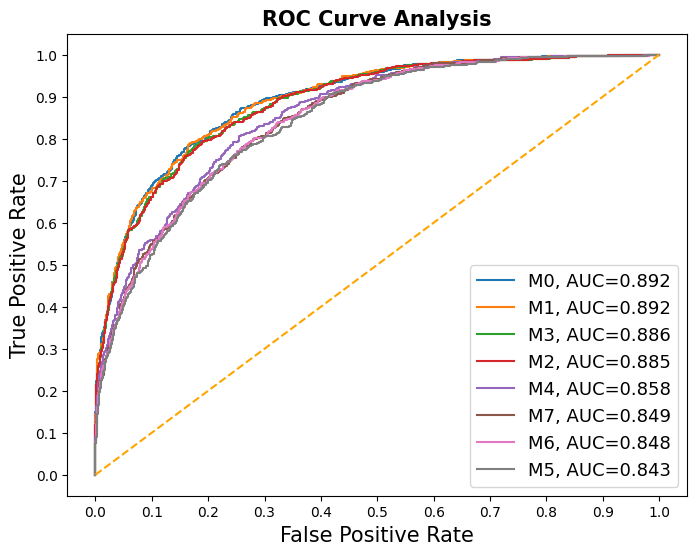
\includegraphics[width=\textwidth]{imatges/results/rocaucanalysis-all.png}
  \caption[ROC-AUC Results in Test Dataset]{\textit{ROC-AUC Results in Test Dataset. }}
  {\label{fig:rocaucanalysis-all}}
\end{figure}

\newpage


\section{Micro-services Communication}

The communication between the API and UI service is facilitated by the HTTP
protocol, which enables responsiveness and scalability within our
infrastructure. To handle long-running tasks in the background effectively, we
have implemented a solution that ensures the system remains highly responsive.
\\

Our approach involves allowing clients to initiate tasks and receive a unique
identifier for each initiated task. When a client initiates a task, the API
micro-service allocates a separate thread to run the task in the background.
The API then returns a unique task identifier that represents this background
task (Figure \ref{fig:backgrond-task}). \\

With this unique task identifier, clients can later query the results of the
asynchronous task. By adopting this method, we avoid congesting the API thread,
ensuring smooth and efficient handling of multiple tasks concurrently. This
mechanism contributes to the overall responsiveness and scalability of our
infrastructure.

\begin{figure}[H]
  \centering
  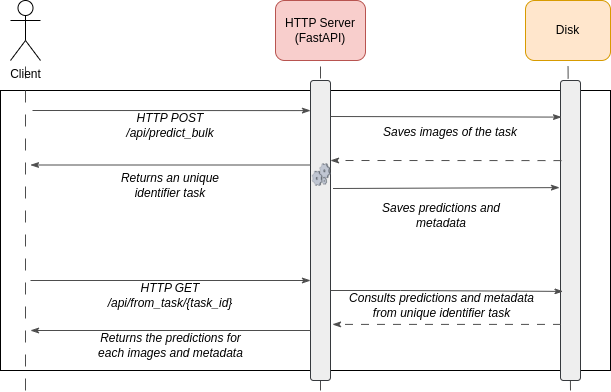
\includegraphics[width=0.9\textwidth]{imatges/preliminaries/BackgroundTask.drawio.png}
  \caption[Inferring Images Through the Background Task Mechanism]{\textit{Inferring Images Through the Background Task Mechanism.  }}
  {\label{fig:backgrond-task}}
\end{figure}

\newpage

\section{API Service}

The API service provides various endpoints accessible through the following URL:

\begin{Verbatim}[fontsize=\scriptsize]
http://<api>/docs
\end{Verbatim}

By opening this URL in a web browser, you can visualize the supported endpoints of the API
(Figure \ref{fig:api-endpoints}). This convenient visualization is made possible by using fastAPI,
the framework chosen for building the API, which operates on the OpenAPI scheme.

\begin{figure}[H]
  \centering
  \begin{adjustbox}{width=\textwidth, trim={0.2cm 0cm 0.1cm 0cm}, clip}
    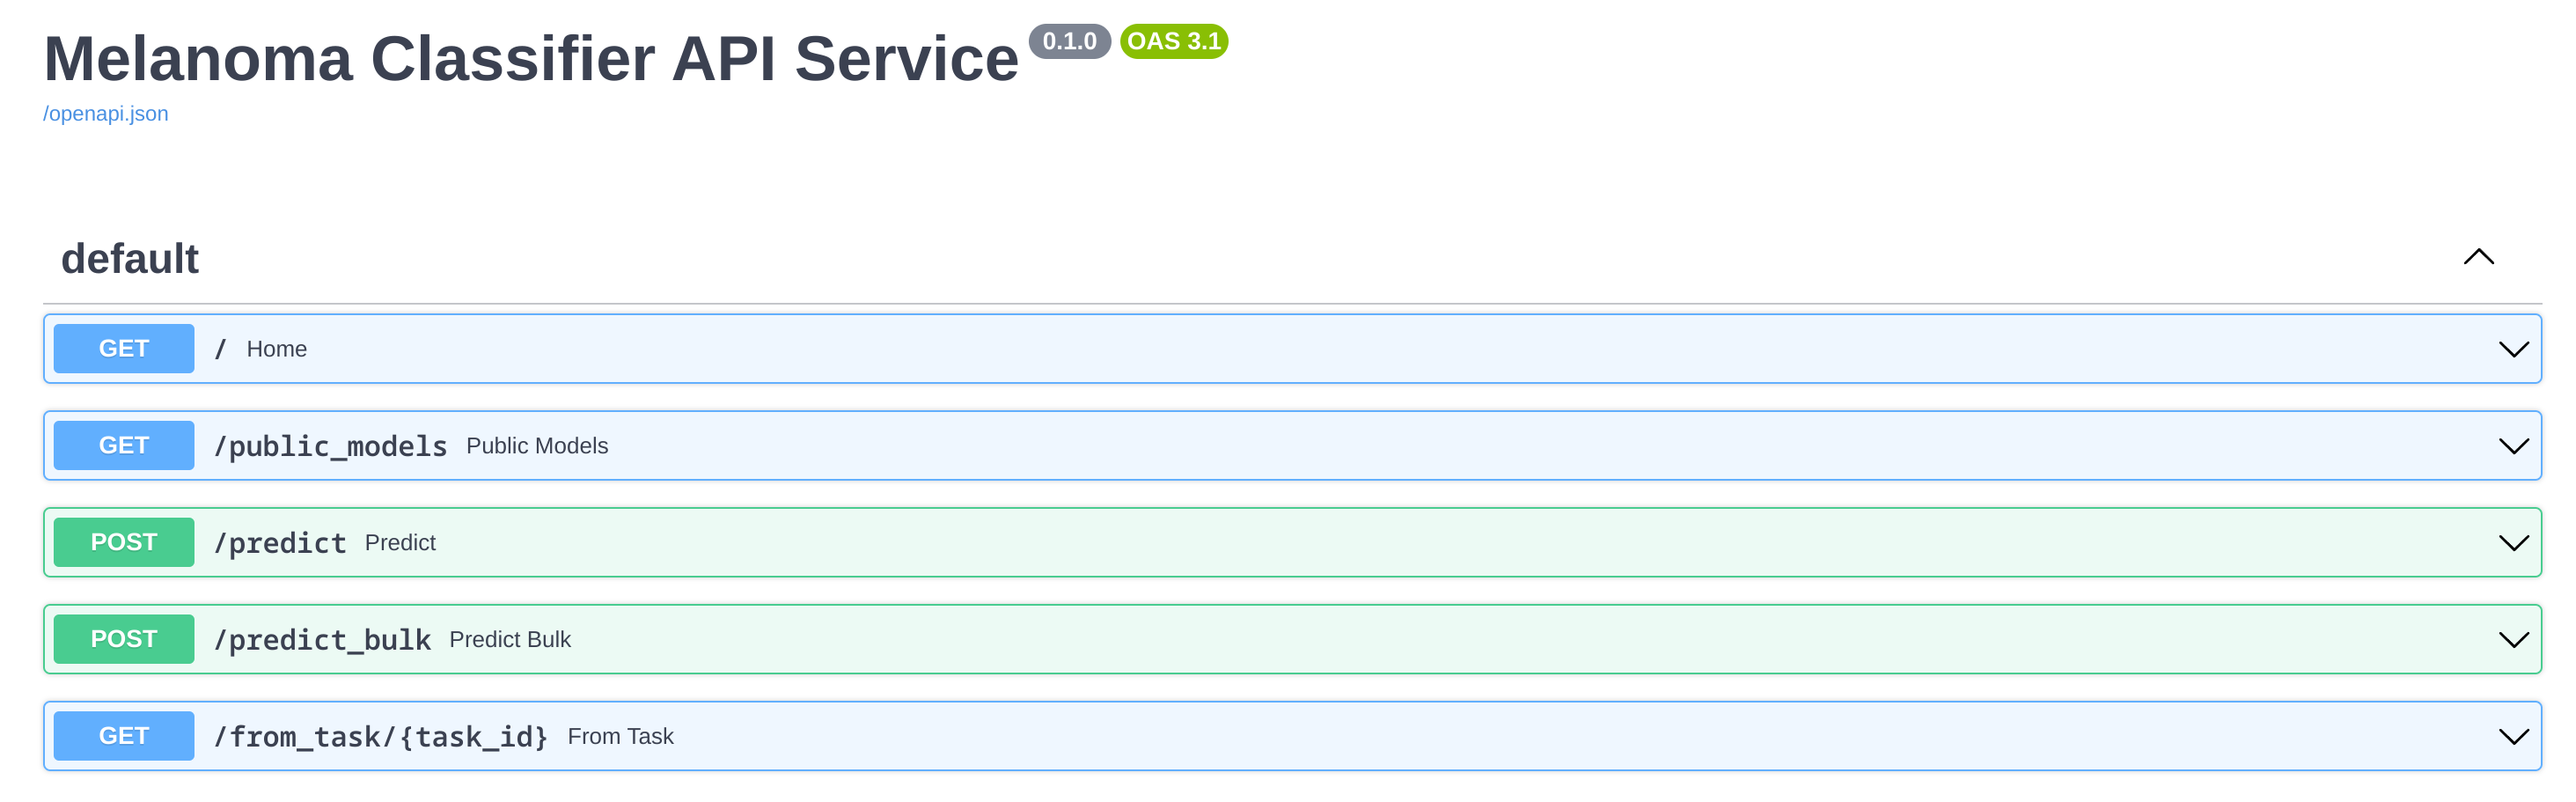
\includegraphics[width=\textwidth]{imatges/results/api-endpoints.png}
  \end{adjustbox}
  \caption[API Service End-Points]{\textit{API Service End-Points. }}
  {\label{fig:api-endpoints}}
\end{figure}

Below, we present an explanation of the functionality of each use case and it's
end-point along with a brief code summary. However, for a comprehensive
understanding of the implementation, we highly recommend referring to the
source code attached to the thesis.

\subsection{Consulting The Available Models}

We provided a mechanism to consult the available models that currently the API
exposes. The supported model are configured in the configuration file of the
API. \\

You can consult the exposed models by requesting:

\begin{Verbatim}[fontsize=\scriptsize]
http://<api>/public_models
\end{Verbatim}

The response of the API's JSON response should be something similar to this:

\begin{Verbatim}[fontsize=\scriptsize]
{
  "models": [
    "M0",
    "M1",
    "M2",
    "M3",
    "M4",
    "M5",
    "M6",
    "M7",
    "vicorobot.8c_b3_768_512_18ep_best_20_fold0",
    "vicorobot.8c_b3_768_512_18ep_best_fold0",
    "vicorobot.8c_b3_768_512_18ep_final_fold0"
  ]
}
\end{Verbatim}



\subsection{Predict an Image}

To predict an individual image, an endpoint is created.
This endpoint expects an HTTP request containing a JPEG image in the body,
along with the specified model name for performing the inference. \\

For example, a valid request to this endpoint might look like:

\begin{Verbatim}[fontsize=\scriptsize]
POST http://<api>/predict?model_id=M1
\end{Verbatim}

The API will respond with a JSON object containing a unique task identifier:

\begin{Verbatim}[fontsize=\scriptsize]
{
  "task_uuid": "721445f5-ff37-4c99-af74-7157925b4a7c"
}
\end{Verbatim}


\subsection{Predict a Jar of Images}

This endpoint is designed to handle requests for predicting multiple images
simultaneously. The main distinction is that this endpoint has the capability
to run the predictions in separate threads. This prevents the system from
becoming unresponsive or stuck while predicting a large number of images, as it
allows the processing to occur concurrently and independently of the main
system thread. \\

To utilize this endpoint, you are required to provide two pieces of information
in the HTTP request: the model you wish to use for image inference and a list
of images attached to the request body. For example, you can use this endpoint
as follows:

\begin{Verbatim}[fontsize=\scriptsize]
http://<api>/predict_bulk?model_id=M1
\end{Verbatim}

The API will respond with a JSON object containing a unique task identifier
and the total number of images sended to the API:

\begin{Verbatim}[fontsize=\scriptsize]
{
  "task_uuid": "77d5e834-60a1-49b6-a71a-b3472dc21ce5",
  "num_images": 2
}
\end{Verbatim}


\subsection{Consulting Task Predictions}

Lastly, we needed and end-point that given the unique identifier task,
we could consult the result of the prediction of the models for all images
sended to the API. \\

You can consult a task prediction as follow:

\begin{Verbatim}[fontsize=\scriptsize]
http://<api>/from_task/77d5e834-60a1-49b6-a71a-b3472dc21ce5
\end{Verbatim}

A potential JSON response from the API regarding the task prediction inquiry
could be:

\begin{Verbatim}[fontsize=\scriptsize]
[
  {
    "name": "ISIC_0052349.jpg",
    "probabilities": {
      "AK": 0.0007466986,
      "BCC": 0.0005002805,
      "BKL": 0.015733117,
      "DF": 0.00086343783,
      "SCC": 0.0007902466,
      "VASC": 0.0017217622,
      "melanoma": 0.017426228,
      "nevus": 0.9622182
    },
    "metadata": {
      "origin": "wilberquito",
      "net_type": "resnet18",
      "img_size": 256,
      "out_dim": 8
    },
    "prediction": {
      "target": false,
      "label": 7,
      "prediction": "nevus"
    }
  },
  {
    "name": "ISIC_1766619.jpg",
    "probabilities": {
      "AK": 0.00016253705,
      "BCC": 0.00011373816,
      "BKL": 0.00052201655,
      "DF": 0.0006251502,
      "SCC": 0.00032183932,
      "VASC": 0.00025595966,
      "melanoma": 0.0012655357,
      "nevus": 0.9967333
    },
    "metadata": {
      "origin": "wilberquito",
      "net_type": "resnet18",
      "img_size": 256,
      "out_dim": 8
    },
    "prediction": {
      "target": false,
      "label": 7,
      "prediction": "nevus"
    }
  }
]
\end{Verbatim}

\section{UI Service}

The UI service plays a crucial role in the CAD infrastructure as it serves as
the interface for interacting with health professionals. In this section, we
highlight some of the most interesting features provided by this service.

Upon accessing the UI service through your web browser, you will immediately
notice a single-page web application with several interactive buttons, as
depicted in Figure \ref{fig:ui-tools}.

\begin{figure}[H]
  \centering
  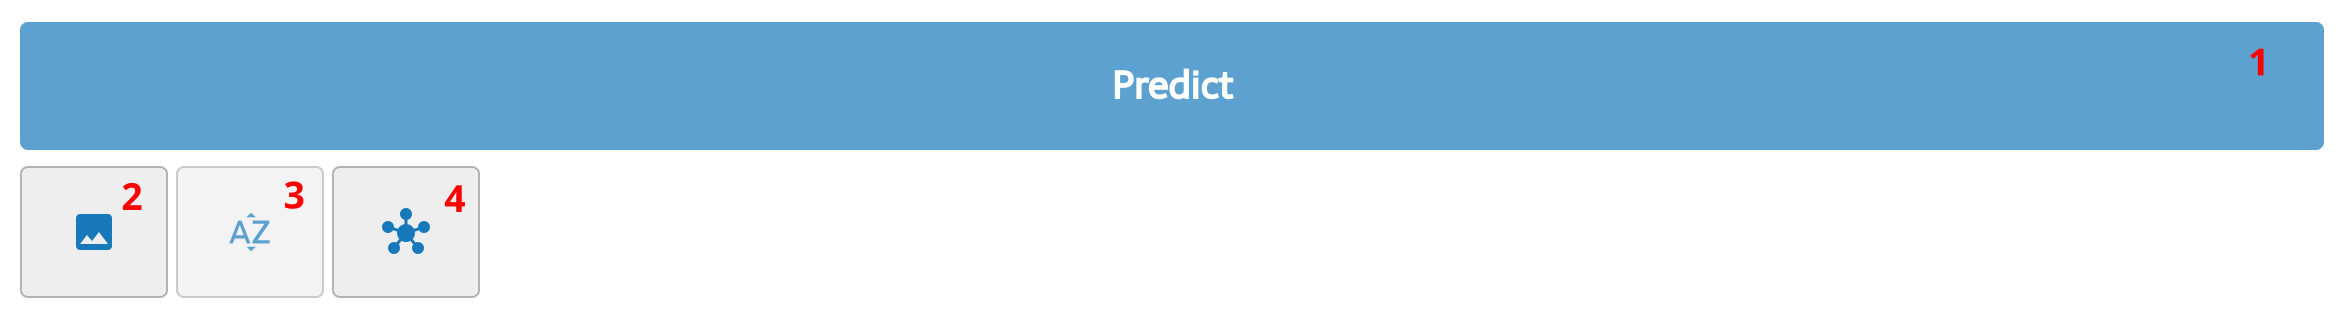
\includegraphics[width=\textwidth]{imatges/results/ui-tools.png}
  \caption[Main Interactive buttons of the UI Service]{\textit{Main Interactive buttons of the UI Service. }}
  {\label{fig:ui-tools}}
\end{figure}

The numbered buttons in Figure \ref{fig:ui-tools} serve the following
main functionalities:

\begin{itemize}
  \item 1. This button serves a dual purpose based on the UI's current state. Firstly, it allows users to initiate a prediction request when they have selected the desired images. Secondly, it serves to reset the UI for the next request, clearing any previously loaded images.
  \item 2. This button enables users to load images directly from their device.
  \item 3. Designed to sort the loaded images in the UI, this button operates differently depending on whether the inference has been performed. If the inference has not been executed, it sorts the images by name. However, if the inference results have been obtained from the API, the button sorts the images by importance, prioritizing melanoma classifications followed by others.
  \item 4. This button displays a list of models exposed by the API. Users can select one of these models to serve as the primary model for the inference in the prediction request.
\end{itemize}


The first thing we would like to do is to load the desired images to make the
prediction. But we can notice that in the state of no having image loaded some
of this buttoms are disabled. When no image is loaded the prediction and the
sort buttom are disabled. \\

To load the desired dermoscopy images we click the button that allows us load
images and select the images from our device
(Figure \ref{fig:selecting-imgs}).

\begin{figure}[H]
  \centering
  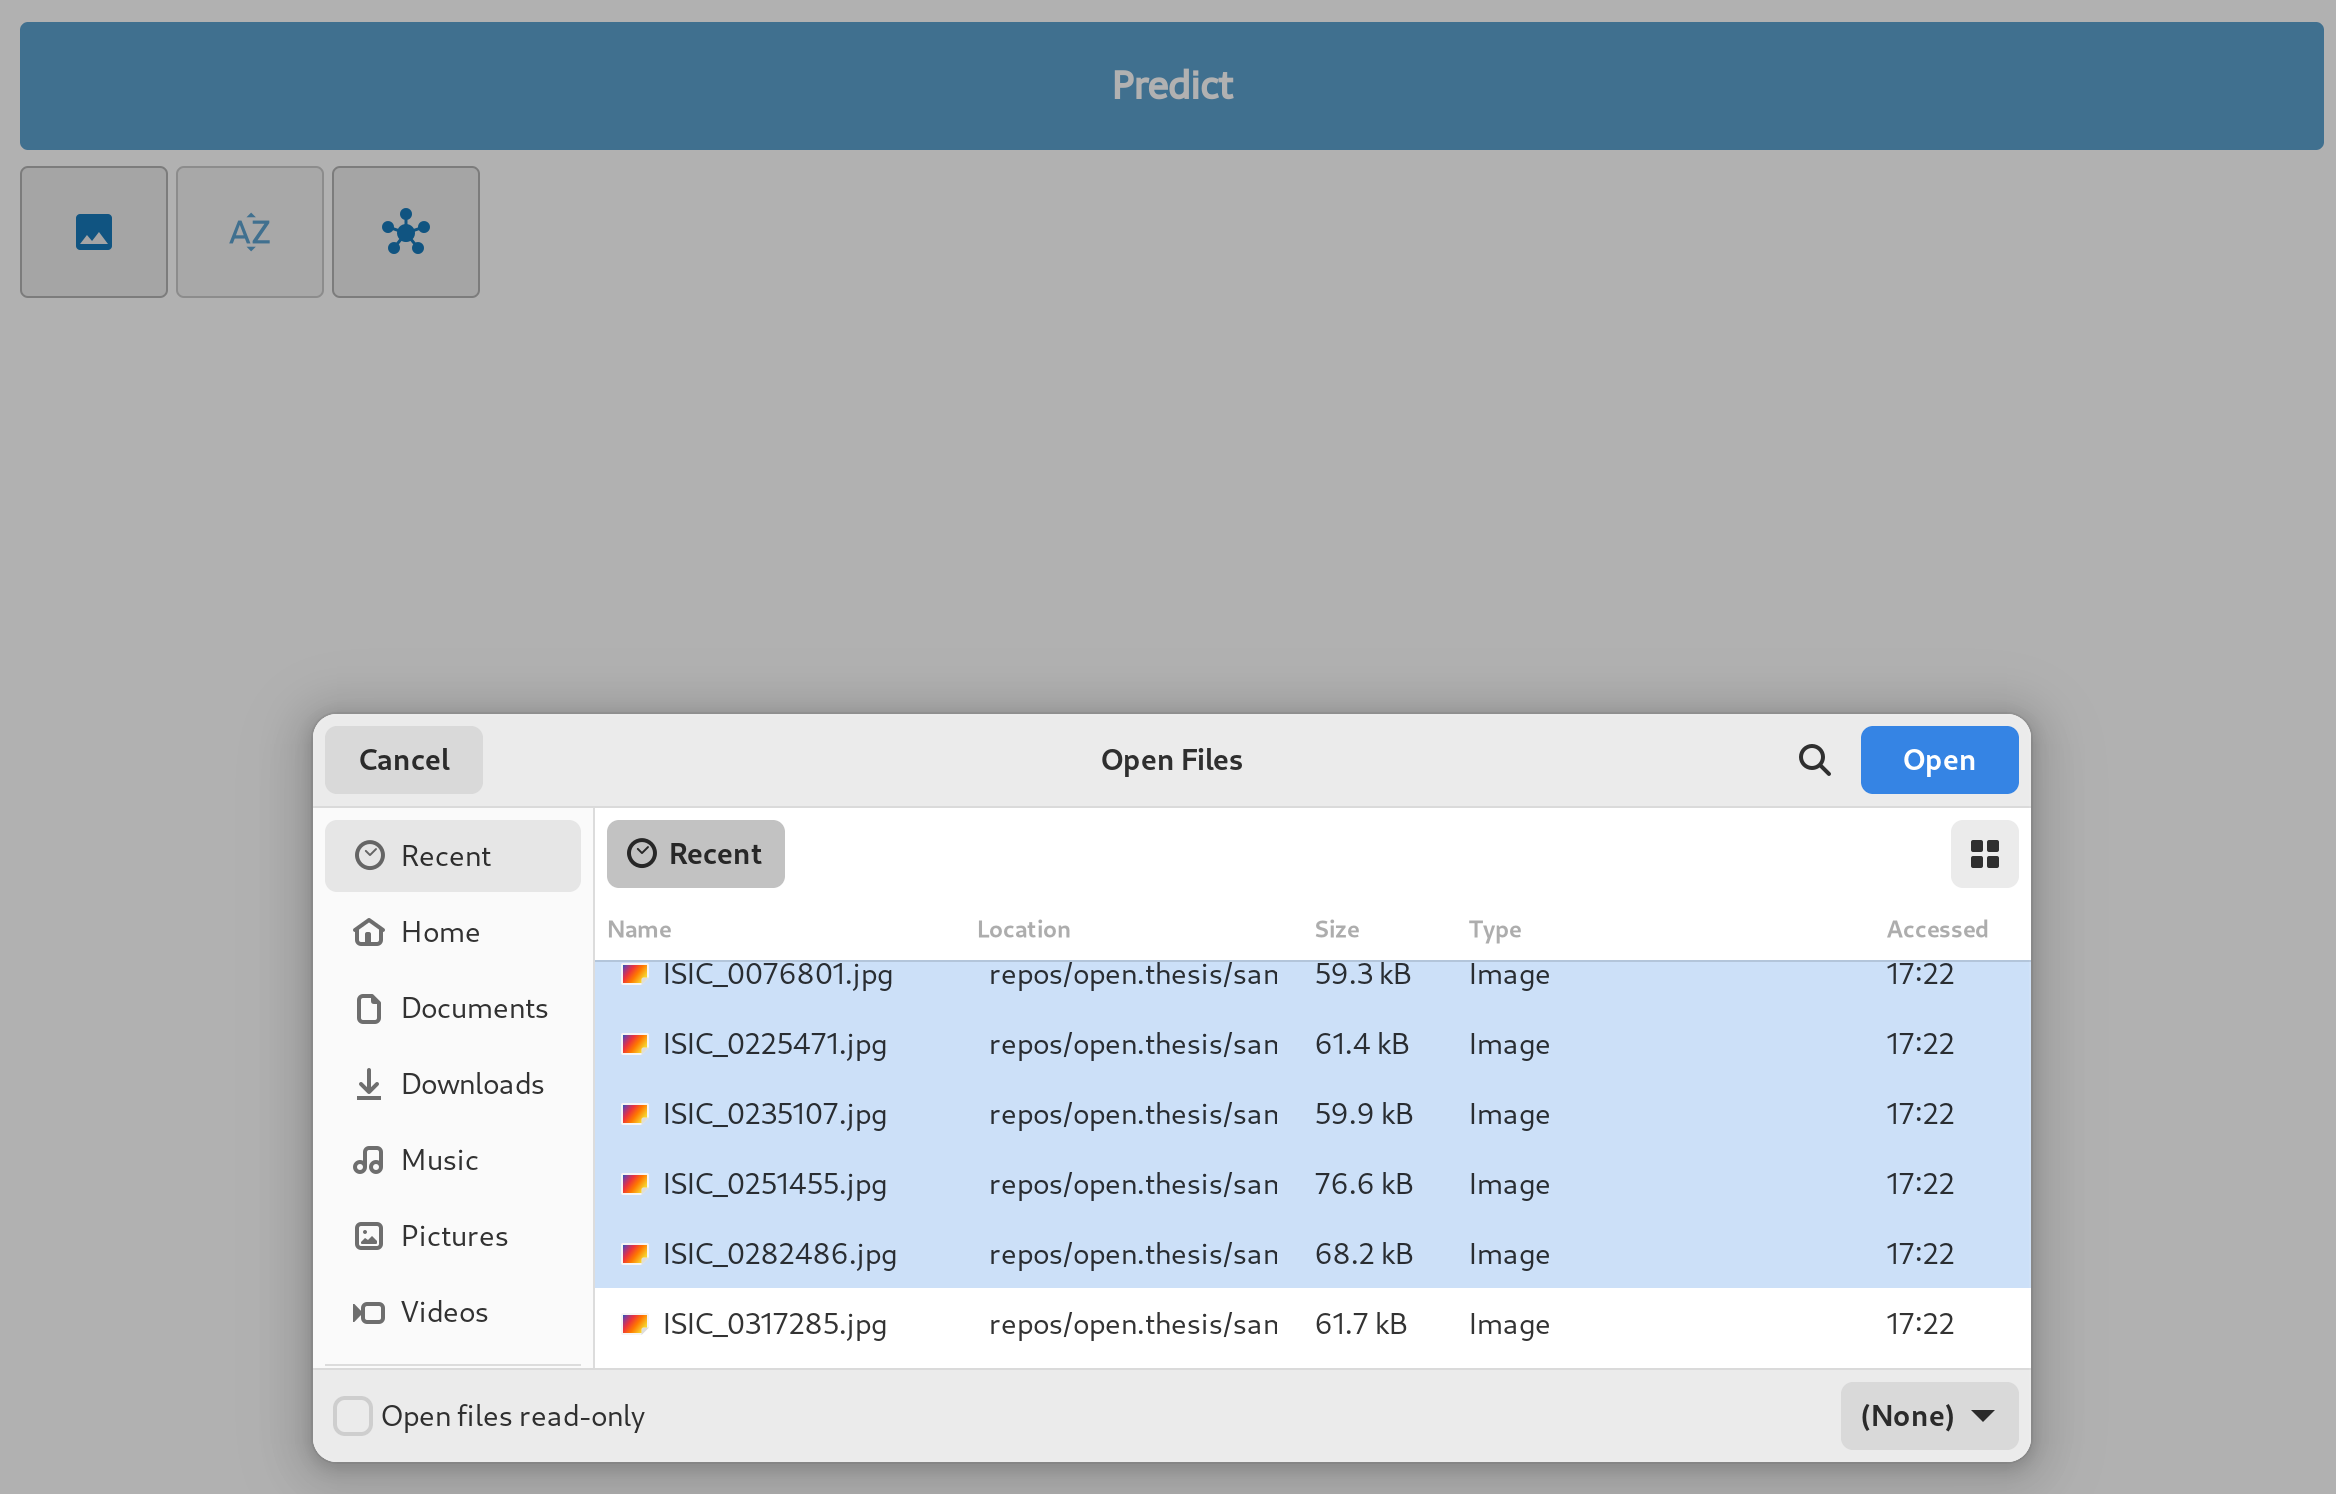
\includegraphics[width=\textwidth]{imatges/results/selecting-images.png}
  \caption[Loading Dermoscopy Images From Device]{\textit{Loading Dermoscopy Images From Device. }}
  {\label{fig:selecting-imgs}}
\end{figure}

After selecting the images, they will be shown in a scrollable section within
the UI service (Figure \ref{fig:loaded-images}), at this point you can
unload any image clicking to the cross in the top-right corner of each image.
You will also notice that the sorting button is now available, along with the
prediction button. Before making any predictions, there is an option to change
the model for inference. By clicking on the "Select Model" button, a scrollable
section will appear next to the working button tools (Figure
\ref{fig:selecting-model}). This allows us to easily switch between different
models for the prediction process.

\begin{figure}[H]
  \centering
  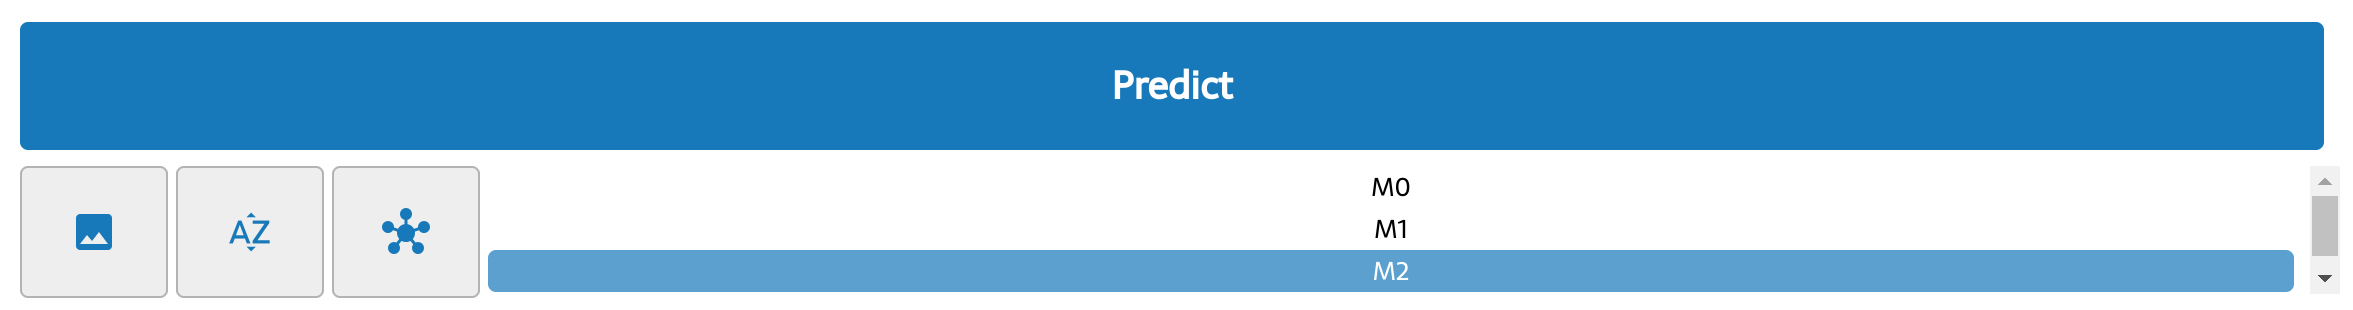
\includegraphics[width=\textwidth]{imatges/results/selecting-model.png}
  \caption[Selecting Exposed Models by the API]{\textit{Selecting Exposed Models by the API. }}
  {\label{fig:selecting-model}}
\end{figure}


\begin{figure}[H]
  \centering
  \begin{adjustbox}{width=\textwidth, trim={0cm 3.5cm 0cm 0cm}, clip}
    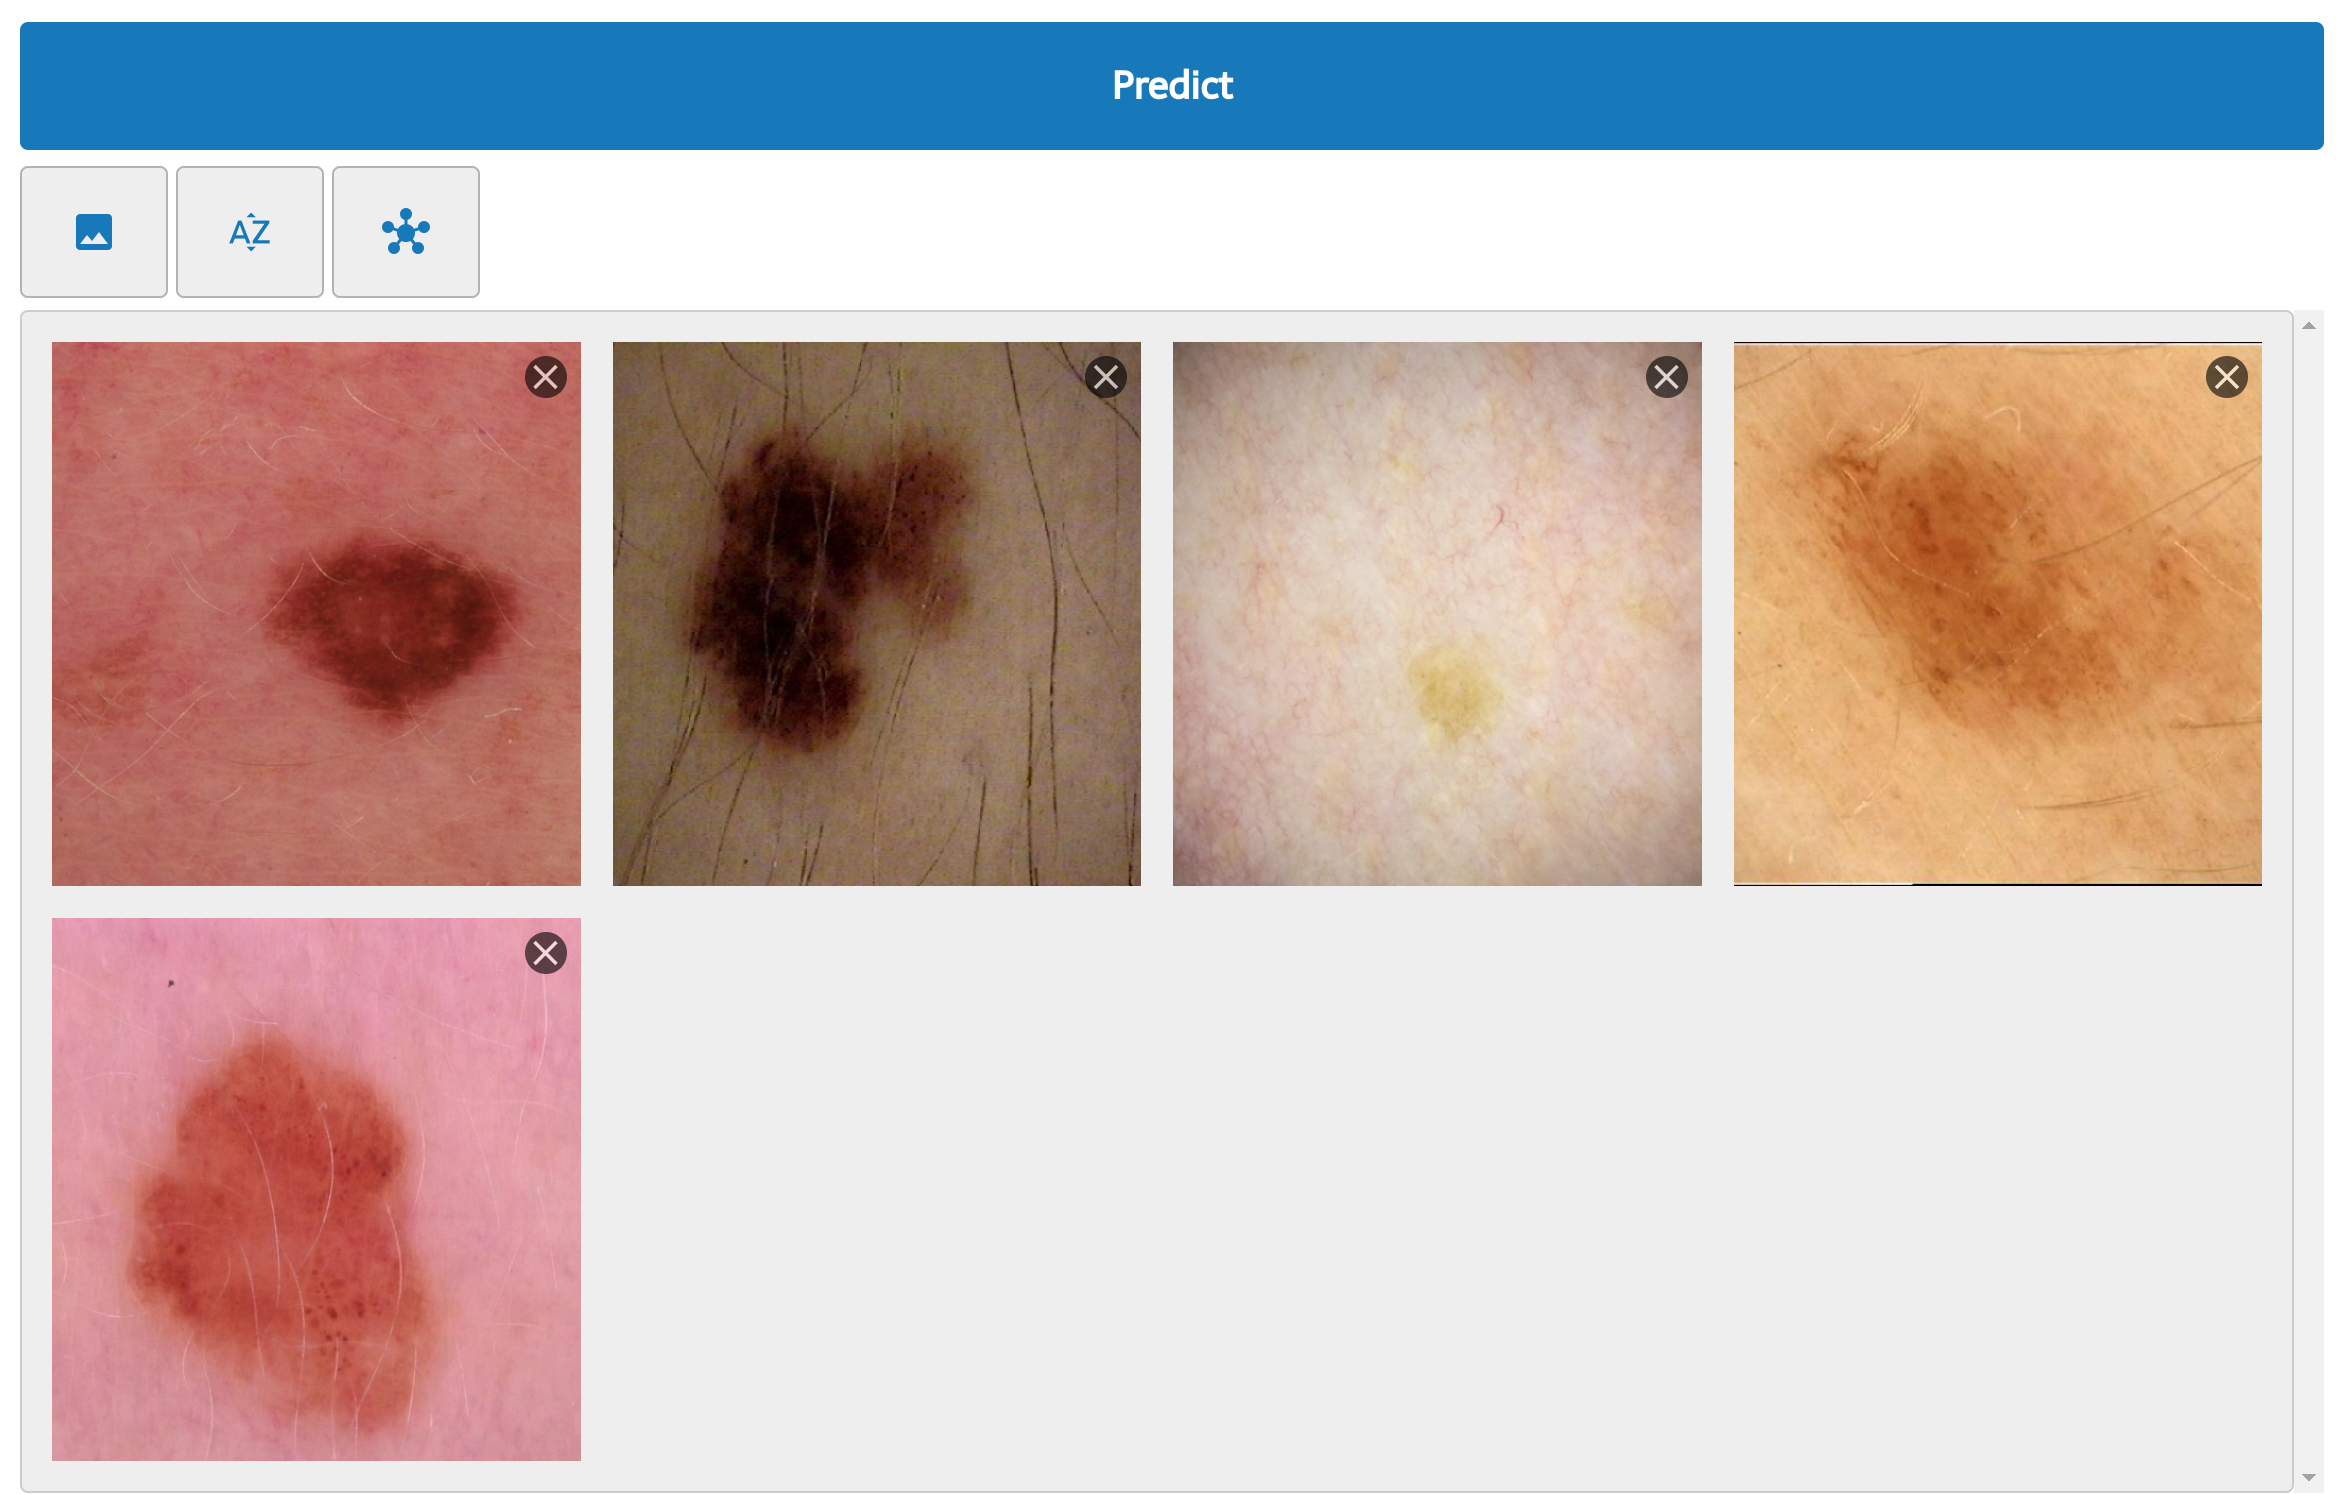
\includegraphics[width=\textwidth]{imatges/results/loaded-images.png}
  \end{adjustbox}
  \caption[Dermoscopy Images Loaded in the UI]{\textit{Dermoscopy Images Loaded in the UI. }}
  {\label{fig:loaded-images}}
\end{figure}

Once we have loaded the images and selected the desired model for prediction,
we are ready to make the request to the API for inference using the chosen model. When the API responds,
the UI will display the images classified as melanoma with a
red background and the images classified as other classes with a blue background (Figure \ref{fig:after-prediction}).
This visual distinction helps to easily identify the different classifications provided by the inference process.

\begin{figure}[H]
  \centering
  \begin{adjustbox}{width=\textwidth, trim={0cm 3.55cm 0cm 0cm}, clip}
    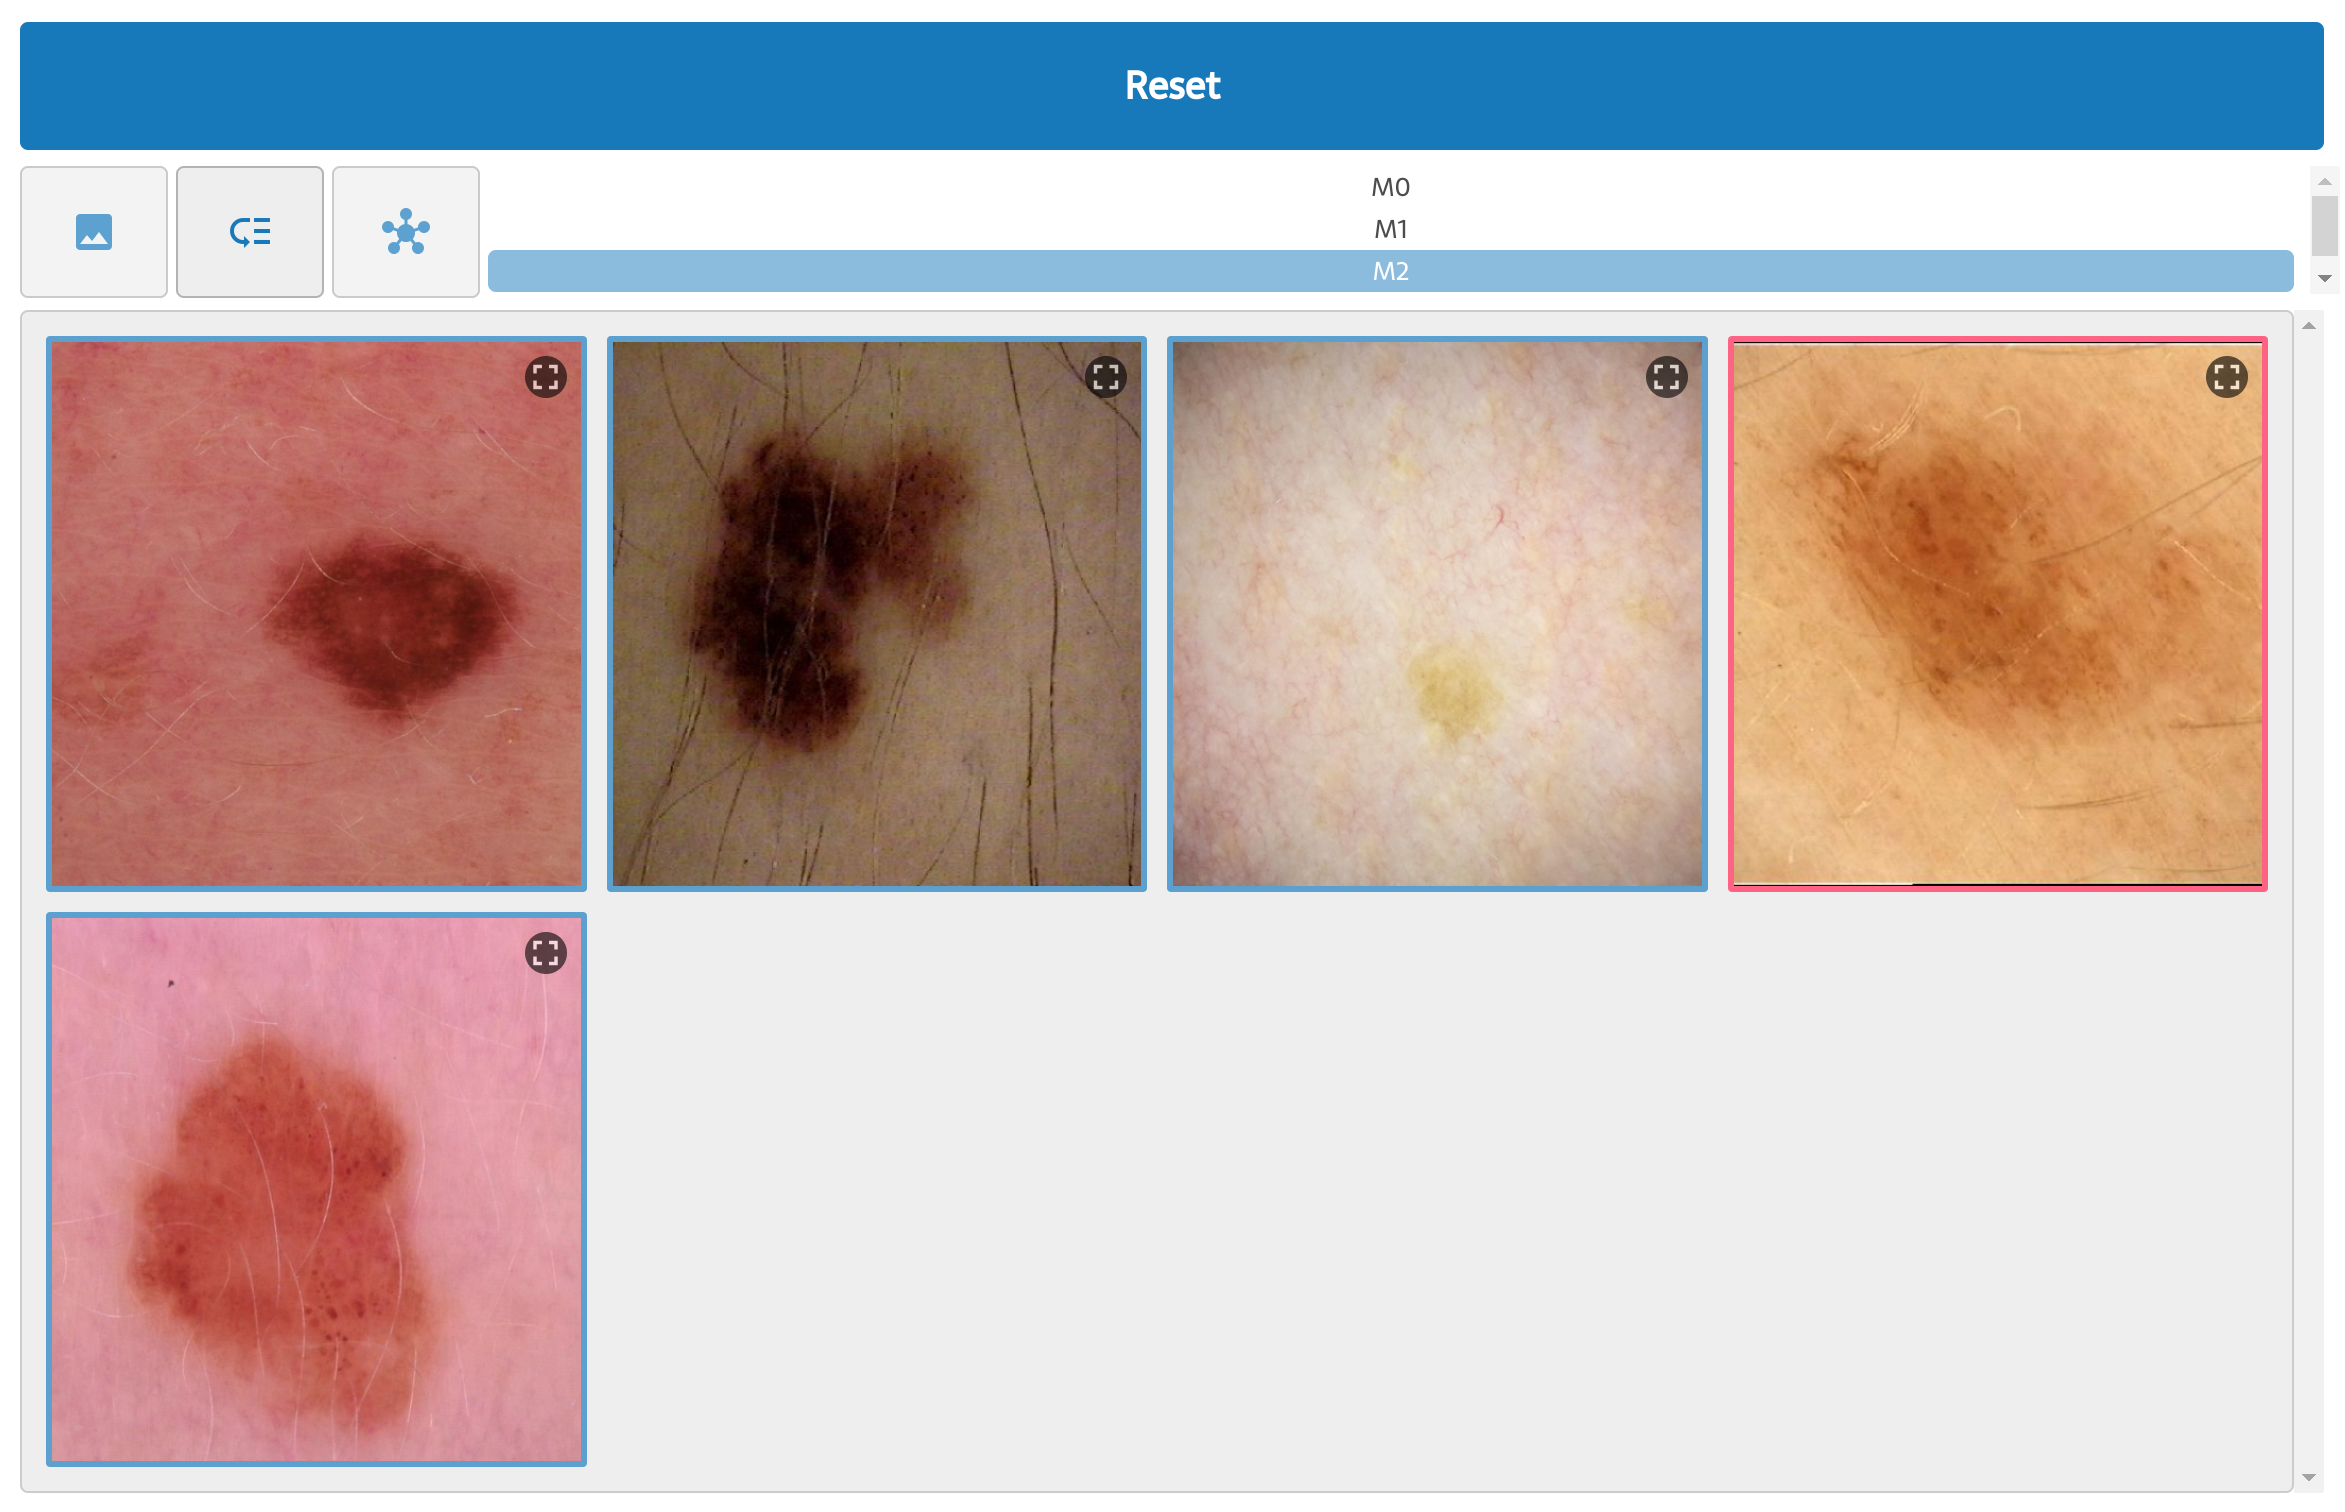
\includegraphics[width=\textwidth]{imatges/results/after-prediction.png}
  \end{adjustbox}
  \caption[UI State After Prediction Response]{\textit{UI State After Prediction Response. }}
  {\label{fig:after-prediction}}
\end{figure}

In this state, all images in the top-right corner feature a button with a
square symbol. When you click on any of these buttons, a pop-up window appears,
providing additional information about the prediction for that specific image.
The pop-up displays the image itself, meta-data regarding the model used for
the prediction, the predictions made, and the probability of the dermoscopy
image belonging to each possible class. \\

For instance, let's inquire about more information on the only image classified
as melanoma in Figure \ref{fig:after-prediction}. Clicking on the
corresponding button will trigger a pop-up, as depicted in Figure
\ref{fig:extra-inf-popup}, showcasing the relevant details for that particular
prediction.

\begin{figure}[H]
  \centering
  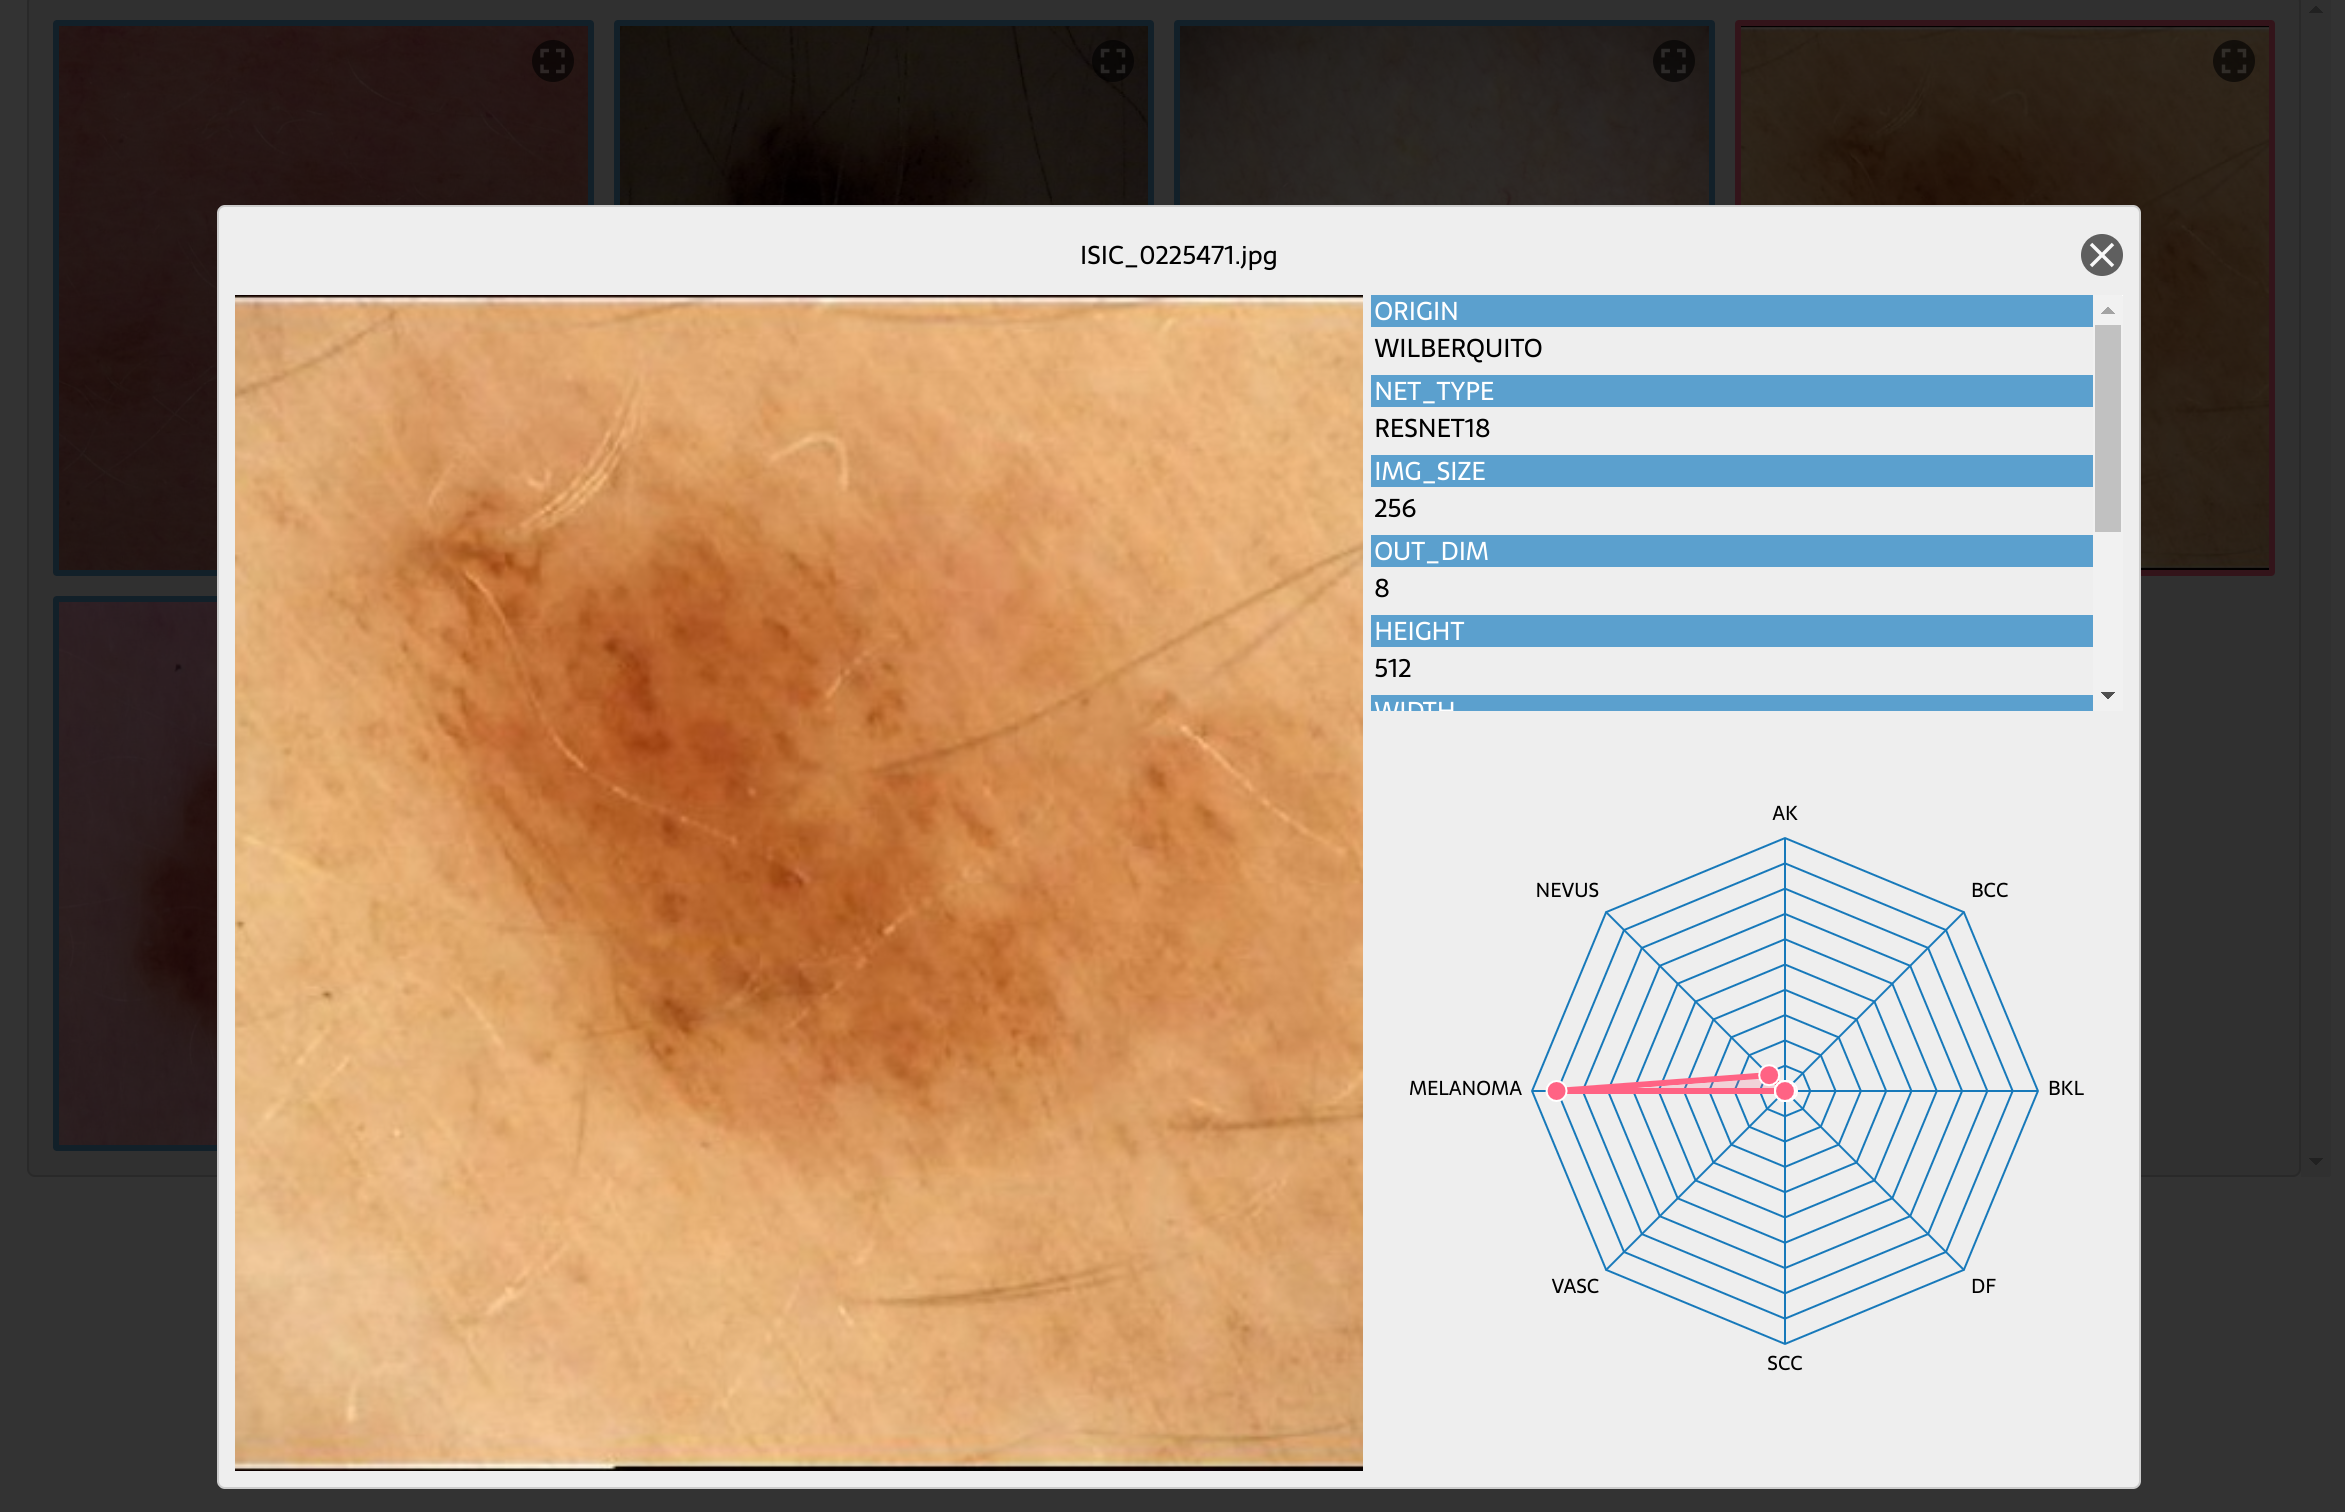
\includegraphics[width=\textwidth]{imatges/results/extra-inf-popup.png}
  \caption[Pop-up Information For Dermoscopy Prediction]{\textit{Pop-up Information For Dermoscopy Prediction. }}
  {\label{fig:extra-inf-popup}}
\end{figure}
